\documentclass[11pt,a4paper]{article}
\usepackage[margin=2.4cm]{geometry}
\usepackage{amsmath,amssymb,amsthm}
\usepackage{booktabs,array,tabularx,longtable}
\usepackage{graphicx}
\usepackage{float}
\usepackage[section]{placeins}
\graphicspath{{./}{figures/}}
\usepackage{enumitem}
\usepackage{xurl}
\usepackage[colorlinks=true,urlcolor=blue,linkcolor=blue,citecolor=blue]{hyperref}
\usepackage[authoryear,round]{natbib}
\emergencystretch=3em
\setlength{\tolerance}{2000}

\renewcommand{\thesection}{S\arabic{section}}
\renewcommand{\theequation}{S\arabic{equation}}
\renewcommand{\thetable}{S\arabic{table}}
\renewcommand{\thefigure}{S\arabic{figure}}
\newtheorem{proposition}{Proposition}
\renewcommand{\theproposition}{S\arabic{proposition}}
\newtheorem{lemma}{Lemma}
\renewcommand{\thelemma}{S\arabic{lemma}}
\newcommand{\pos}[1]{\left[#1\right]_+}
\newcommand{\dconv}{\Delta b_{\mathrm{conv}}}
\newcommand{\Ups}{\Upsilon_c}
\newcommand{\Eceil}{E_{\mathrm{ceil}}}
\newcommand{\Acmin}{A_c^{\min}}
\newcommand{\tconv}{\tau_{\mathrm{conv}}}

\title{Supplementary Information for\\[4pt]
\large A rising biocapacity total can mask ecological-capital land drawdown: a two-land model}
\author{Amin Abaee\\ \small Independent Researcher, Tehran, Iran\\ \small \href{mailto:amin_abaee@ut.ac.ir}{amin\_abaee@ut.ac.ir} \quad\href{https://orcid.org/0000-0002-0019-1842}{ORCID 0000-0002-0019-1842}}

\date{}

\begin{document}
\maketitle

\noindent Equation numbers without the prefix S refer to the main text.

\section{Symbols and model extensions}\label{si:symbols}

A global hectare (gha) adjusts a hectare to world-average biological productivity for the relevant account year. Annual Ecological Footprint and biocapacity flows are reported in gha, with the annual basis implicit in that year \citep{GFNStandards2009,GFNGuidebook2019}. In the model, $B$ and $E$ are annual account-equivalent quantities; in the empirical analysis, $B$ and $E_{\mathrm{prod}}$ are observed NFA account values. Model contributions $Y_f$ and $Y_c$ and shortfall $S$ use the same units, but are not separate NFA series. The debt state $D$ is a leaky state driven by aggregate deficit $E-B$ and is measured in gha\,yr; $\dot D$ and $\eta D$ are in gha.

\begin{longtable}{>{\raggedright\arraybackslash}p{0.12\textwidth}>{\raggedright\arraybackslash}p{0.41\textwidth}>{\raggedright\arraybackslash}p{0.2\textwidth}>{\raggedright\arraybackslash}p{0.14\textwidth}}
\caption{Symbols, definitions, units, and roles. Per-hectare yields and contributions use the annual account basis (gha\,ha$^{-1}$). The coefficient $b_{G,c}$ is in gha\,yr\,ha$^{-1}$; annual account totals are in gha, with the accounting year implicit. The leaky debt state $D$ is in gha\,yr.}\label{tab:si_symbols}\\
\toprule
Symbol & Meaning & Unit & Role \\
\midrule
\endfirsthead
\toprule
Symbol & Meaning & Unit & Role \\
\midrule
\endhead
$A_f$ & fast provisioning land (cropland, intensive) & ha & state \\
$A_c$ & ecological-capital land (forest, soil, wetland, long-rotation systems; effective class) & ha & state \\
$A_r$ & reserve land, $A_{tot}-A_f-A_c$ & ha & dependent balance \\
$q$ & uncalibrated, model-defined capital-land quality index & dimensionless & state \\
$K_q$ & admissible quality set, $[0,q_{\max}]$ & dimensionless & imposed interval \\
$P$ & human population & cap & state \\
$D$ & leaky-debt state driven by aggregate deficit $E-B$ & gha\,yr & state \\
$b_f$ & fast-land account yield per hectare, $(b_{f0}+T_b)e^{-\alpha D}$ & gha\,ha$^{-1}$ & derived \\
$\tilde b_f(t)$ & OWID/FAOSTAT cereal yield, a physical productivity indicator (not all crops) & tonnes\,ha$^{-1}$ & empirical input \\
$\hat b_f(t)$ & Base-anchored index-scaled proxy yield used only in SI S5 & gha\,ha$^{-1}$ & proxy construction \\
$b_{f0}$ & base fast-land yield per hectare & gha\,ha$^{-1}$ & parameter \\
$b_c$ & capital-land direct yield & gha\,ha$^{-1}$ & parameter \\
$b_{G,c}$ & capital regeneration-value coefficient & gha\,yr\,ha$^{-1}$ & parameter \\
$G_c(q)$ & per-ha regeneration of quality, $\rho_cq(1-q/q_{\max})$ & yr$^{-1}$ & rate function \\
$\Ups(q)$ & per-ha capital value, $b_c+b_{G,c}G_c(q)$ (also written $b_{c,\mathrm{eff}}$) & gha\,ha$^{-1}$ & derived \\
$\dconv$ & composition diagnostic, $b_f-\Ups(q)$ & gha\,ha$^{-1}$ & derived \\
$Y_f,\ Y_c$ & fast and capital yields, $b_fA_f$ and $\Ups A_c$ & gha & derived \\
$B$ & model biocapacity $Y_f+Y_c$; or NFA total under its account convention & gha & aggregate \\
$E_{\mathrm{prod}}$ & NFA Global Ecological Footprint of Production & gha & empirical account \\
$E$ & model-defined footprint demand, $eP$ (or exogenous fixed demand) & gha & aggregate \\
$X,\ C$ & crop-proxy account $X=\hat b_fA_f$ and residual $C=B-X$; neither is physical capital & gha & illustrative accounting split \\
$S$ & shortfall, $\pos{E-\sigma_fY_f-\sigma_cY_c}$ & gha & derived \\
$u_c$ & conversion rate, $\min(S/b_f,\,A_c-\Acmin)/\tconv$ & ha\,yr$^{-1}$ & flow \\
$K$ & carrying capacity, $\max(B/e,K_{\min})$ & cap & algebraic \\
$e$ & per-capita footprint & gha\,cap$^{-1}$ & parameter \\
$r$ & intrinsic population growth rate & yr$^{-1}$ & parameter \\
$\rho_c$ & quality-regeneration scenario rate & yr$^{-1}$ & scenario parameter; not estimated \\
$q_{\max}$ & imposed quality admissibility bound & dimensionless & not an estimated threshold \\
$\mu$ & cropland maintenance rate (reserve$\to$fast) & yr$^{-1}$ & parameter \\
$\eta_f$ & fast-land retirement rate (fast$\to$reserve) & yr$^{-1}$ & parameter \\
$\tconv$ & conversion time constant & yr & parameter \\
$\alpha$ & degradation rate of $b_f$ per unit debt in the multiplicative law & gha$^{-1}$\,yr$^{-1}$ & parameter \\
$\alpha_{\mathrm{add}}$ & coefficient in the additive comparator $b_f=b_{f0}+T_b-\alpha_{\mathrm{add}}D$ & ha$^{-1}$\,yr$^{-1}$ & comparator only; distinct from $\alpha$ \\
$\eta$ & debt-repayment rate & yr$^{-1}$ & parameter \\
$\tau_g,\ \tau_p$ & regeneration and demographic delay scenarios & yr & scenario parameters \\
$\sigma_f,\ \sigma_c$ & human-available shares of the two flows & dimensionless & parameter \\
$R_{rc}$ & surplus-gated restoration, $\chi_rA_r\pos{B-E}$ (reserve$\to$capital) & ha\,yr$^{-1}$ & gated flow \\
$\chi_r$ & restoration coefficient & gha$^{-1}$\,yr$^{-1}$ & parameter \\
$T_b$ & technology yield increment, $\omega_{Tb}\Delta b/(1+e^{-\kappa_w(t-t_{wave})})$ & gha\,ha$^{-1}$ & off except in SI S8 \\
$\omega_{Tb}$ & activation flag for the technology wave & dimensionless & $0$ baseline; $1$ in SI S8 \\
$\Delta b$, $\kappa_w$, $t_{wave}$ & amplitude, steepness and center of the wave & gha\,ha$^{-1}$;\newline yr$^{-1}$; yr & active only in SI S8 \\
$\Acmin$ & capital-land area floor & ha & enforced by conversion-rate law \\
$A_r^{\min}$ & reserve monitoring threshold ($0.10$) & ha & monitored post hoc, not enforced \\
$A_f^{\max}$ & optional fast-land ceiling & ha & not active in reported runs \\
$K_{\min}$ & carrying-capacity floor & cap & imposed in definition of $K$ \\
$A_{tot}$ & total bioproductive area & ha & parameter \\
$k$ & $\mu/(\mu+\eta_f)$, fast share of non-capital land at equilibrium & dimensionless & derived \\
$B_{eq}(A_c)$ & maintenance-balanced land relation; equality at $B_{eq}=E$, with surplus no-conversion states when $B_{eq}>E$ & gha & derived \\
$\Eceil$ & demand ceiling, $B_{eq}(\Acmin)$ & gha & derived \\
$\lambda_{1,2}$ & deficit-side Jacobian eigenvalues & yr$^{-1}$ & derived \\
$R_B,R_A,\psi_f$ & $E/B$, $E/Y_f$, $Y_f/B$ (so $R_A=R_B/\psi_f$) & dimensionless & diagnostics \\
$\phi_0,w_X,w_C$ & base-year cropland share and log-mean weights & dimensionless & empirical decomposition \\
$s_X,\bar s_X,\bar s_C$ & current and average fast-land shares & dimensionless & empirical decomposition \\
$\mathcal R_c(T)$ & recovery metric, $(A_c(T)-A_c^{\mathrm{deg}})/(A_c^{\mathrm{init}}-A_c^{\mathrm{deg}})$ & dimensionless & derived \\
$R_{fc}$, $\chi$ & fast$\to$capital restoration variant, $\chi A_f\pos{B-E}$ & ha\,yr$^{-1}$; gha$^{-1}$\,yr$^{-1}$ & extension (off) \\
$L_c$, $H_c$ & timber liquidation flow $\pos{H_c-\sigma_cY_c}/b_{G,c}$ and its target & ha\,yr$^{-1}$;\newline gha & extension (off) \\
\bottomrule
\end{longtable}

\paragraph{Model extensions.} The reported simulations do not include timber liquidation or direct restoration from fast land to capital land. SI~\S S6 considers reservations of the human-available shares as a policy extension. The technology wave is off in the baseline and gate-sign comparison; it is switched on only for the matched experiment in SI~\S S8.

\paragraph{Conventions.} The positive-part operator is exact, conversion runs at the rate set by $\tconv$, and transfers conserve area across $A_f$, $A_c$, and $A_r$. The quality index $q$ is uncalibrated and model-defined. Its continuous specification is $K_q=[0,q_{\max}]$ and $\dot q(t)=\Pi_{T_{K_q}(q(t))}G_c(q(t-\tau_g))$, where $G_c(x)=\rho_cx(1-x/q_{\max})$, $\rho_c>0$, and $q_{\max}>0$. We use an admissible continuous history $q(s)=\phi(s)\in K_q$ for $s\in[-\tau_g,0]$ and interpret the equation for an absolutely continuous solution almost everywhere. The baseline $q_{\max}=1$ is imposed as an admissibility bound, not an estimated ecological threshold; $\rho_c$ and $\tau_g$ are scenario settings, not estimates from recovery studies. Since $G_c(x)\ge0$ on $K_q$, the quality state is nondecreasing; outward velocity is projected to zero at the upper bound and the lower bound is invariant. Maintenance at rate $\mu A_r$ allows fast-land area to remain positive at equilibrium. The numerical update enforces $A_c\ge\Acmin$, $A_f\ge0$, $q\in K_q$, $P,D\ge0$, and $K\ge K_{\min}$; reserve area is reconstructed from total area, without projection onto $A_r\ge A_r^{\min}$. The reserve threshold is monitored post hoc, not an invariant of the displayed flow. In the reported $\Delta t=0.1$\,yr drawdown grid, the minimum reserve was $0.511$\,ha (initial reserve is $0.72$\,ha for $A_{c0}=1.18$\,ha); the gate-comparison minimum was $0.602$\,ha. These tested values exceed $A_r^{\min}=0.10$\,ha but do not prove invariance. The optional $A_f^{\max}$ ceiling is not imposed in reported runs.

\section{Derivations and proofs}\label{si:proofs}

\subsection{The composition identity with varying debt and quality}\label{si:identity}

Differentiate $B=b_fA_f+\Ups(q)A_c$, use $b_f=(b_{f0}+T_b)e^{-\alpha D}$, and substitute Eqs.~(6)--(7) to obtain the general identity
\begin{equation}\label{eq:si_identity}
\dot B=\dconv\,u_c+b_f\big(\mu A_r-\eta_fA_f\big)+b_{G,c}G_c'(q)A_c\,\dot q+\Ups R_{rc}-\alpha\dot D\,b_fA_f+\frac{\dot T_b}{b_{f0}+T_b}\,b_fA_f .
\end{equation}
The conversion contribution has the sign of $\dconv$. The quality term follows the sign of $G_c'(q)$: it is non-negative for $q\le q_{\max}/2$ and non-positive above that point, since $\dot q\ge0$. While debt accumulates, its contribution is non-positive; a rising technology wave and restoration contribute non-negatively. Proposition~1 in the main text sets $T_b\equiv0$, $R_{rc}\equiv0$, and holds $D$ fixed. In the demonstration run, $D$ instead rises to $0.20\,gha\,yr$ and then declines. Initially, conversion contributes $0.21\,\mathrm{gha\,yr^{-1}}$ to $\dot B$, compared with $-0.005\,\mathrm{gha\,yr^{-1}}$ from fast-land maintenance and retirement and a debt contribution of about $-0.004\,\mathrm{gha\,yr^{-1}}$. Conversion therefore dominates the initial change in aggregate model biocapacity.

\newpage
\subsection{The deficit-side affine system and its spectrum}\label{si:affine}

On the deficit side, set $q=q_{\max}$, freeze $D$, switch off $R_{rc}$, and assume $S/b_f<A_c-\Acmin$. Equation~(5) then gives $u_c=(E-b_fA_f-b_cA_c)/(b_f\tconv)$. Using $A_r=A_{tot}-A_f-A_c$, \mbox{Eqs.~(6)--(7) reduce to}
\begin{equation}
\frac{d}{dt}\begin{pmatrix}A_f\\A_c\end{pmatrix}=
\begin{pmatrix}-\tconv^{-1}-\mu-\eta_f & -\mu-\dfrac{b_c}{b_f\tconv}\\[8pt]\tconv^{-1} & \dfrac{b_c}{b_f\tconv}\end{pmatrix}
\begin{pmatrix}A_f\\A_c\end{pmatrix}+
\begin{pmatrix}\dfrac{E}{b_f\tconv}+\mu A_{tot}\\[8pt]-\dfrac{E}{b_f\tconv}\end{pmatrix}.
\end{equation}
The matrix has trace $\operatorname{tr}J=-\tconv^{-1}(1-b_c/b_f)-\mu-\eta_f$ and determinant $\det J=(\mu+\eta_f)(k-b_c/b_f)/\tconv$, where $k=\mu/(\mu+\eta_f)$. At baseline, $\operatorname{tr}J=-1.0512\,\mathrm{yr}^{-1}$ and $\det J=0.05353\,\mathrm{yr}^{-2}$. Its eigenvalues are
\begin{equation}
\lambda_{1,2}=\tfrac12\Big(\operatorname{tr}J\pm\sqrt{\operatorname{tr}^2J-4\det J}\Big)=-0.0537\,\mathrm{yr}^{-1},\ -0.9975\,\mathrm{yr}^{-1}.
\end{equation}
Because $J$ depends on neither demand $E$ nor the current state, this spectrum stays constant along the fixed-demand deficit-side branch. At $E/\Eceil=0.50,\,0.90,\,0.99,\,0.999$, the slow eigenvalue remains $\lambda_1=-0.05366\,\mathrm{yr}^{-1}$. It is unchanged as $\rho_c$ varies ($\lambda_1=-0.0537\,\mathrm{yr}^{-1}$ at $\rho_c=0.04,\,0.08,\,0.16\,\mathrm{yr}^{-1}$), shifts modestly with $\tconv$ ($-0.0553,\,-0.0537,\,-0.0505,\,-0.0417\,\mathrm{yr}^{-1}$ at $\tconv=0.5,\,1,\,2,\,5\,\mathrm{yr}$), and shifts more with $\mu$ ($-0.0254,\,-0.0537,\,-0.1099\,\mathrm{yr}^{-1}$ at $\mu=0.03,\,0.06,\,0.12\,\mathrm{yr}^{-1}$). It remains negative in every tested sweep.

The affine deficit-side system has the fixed point $A_c^*(E)$ from Eq.~(18), with $A_f^*=k(A_{tot}-A_c^*)$. For $E>\Eceil$, this point lies below $\Acmin$; the trajectory instead approaches $A_c=\Acmin$ asymptotically, with $u_c\to0$ and persistent shortfall $S^*=E-\Eceil$. Separately, in the full endogenous-population model with $K_{\min}$ inactive, a positive stationary population requires $E=B$, so its no-conversion equilibria lie on the equality relation with $P=B/e$. Two such baseline examples are $(A_f^*,A_c^*,A_r^*,P^*)=(0.914\,\mathrm{ha},0.824\,\mathrm{ha},0.762\,\mathrm{ha},1.488\,\mathrm{cap})$ and $(1.091\,\mathrm{ha},0.500\,\mathrm{ha},0.909\,\mathrm{ha},1.731\,\mathrm{cap})$. Both satisfy $A_r^*/A_f^*=\eta_f/\mu=0.8333$; the second is a sustainable cropland equilibrium supported by maintenance. These full-system equality equilibria are distinct from the fixed-demand reduced surplus family ($B_{eq}>E$) and from the one-sided deficit-branch spectrum. The reserve-share mode explains why the strict-inequality interval in the delayed-quality demonstration lasts about $149$\,yr, even though most conversion is complete within $25$\,yr.

When the other branch of the minimum applies ($S/b_f\ge A_c-\Acmin$), $u_c=(A_c-\Acmin)/\tconv$. The distance to the floor then follows $\frac{d}{dt}(A_c-\Acmin)=-(A_c-\Acmin)/\tconv$: it shrinks exponentially but never reaches zero in finite time. The floor is approached asymptotically, so operational proximity thresholds depend on the tolerance used to define “near” (Section~\ref{si:ladder}).

\subsection{Quality-bound and population-delay scope}\label{si:char}

The projected quality law is a constrained delay equation, so the characteristic roots of the raw, unconstrained DDE do not describe its boundary dynamics. For any admissible history and $\rho_c>0$, $G_c(q(t-\tau_g))\ge0$ on $K_q$, and the projected trajectory is nondecreasing. If $q(0)>0$, it has a limit $L\ge q(0)>0$. If $L<q_{\max}$, then $G_c(q(t-\tau_g))\to G_c(L)>0$, contradicting convergence to a finite interior limit; hence $q(t)\to q_{\max}$. The all-zero history remains at zero, so $q_{\max}$ is not a global attractor over every admissible history. We make no characteristic-root stability claim for the projected quality component at the active upper bound.

The population equation delays carrying capacity, not population in its own crowding term. If $K$ is constant, the equation reduces to the ordinary logistic ODE; at a positive equilibrium $P^*=K^*$, its scalar population perturbation satisfies $\delta\dot P=-r\,\delta P$ and has eigenvalue $-r$. With a varying capacity, the local equation at $P^*=K^*$ is $\delta\dot P=-r\,\delta P+r\,\delta K(t-\tau_p)$: the delay is in the capacity input. Thus $r\tau_p<\pi/2$ is not a stability criterion for the equation written in the manuscript. We do not report a full coupled characteristic-root classification for the projected two-land system.

For completeness, on a deficit-active face with $z=(A_f,A_c,q,P,D)$ and $b_f=(b_{f0}+T_b)e^{-\alpha D}$, the debt-state Jacobian row is
\[
\frac{\partial\dot D}{\partial z}=\left(-b_f,-\Ups,-b_{G,c}G_c'(q)A_c,e,\alpha b_fA_f-\eta\right).
\]
In particular, $\partial\dot D/\partial D=\alpha b_fA_f-\eta$; the feedback through $b_f(D)$ is part of the derivative. This row describes the smooth interior of the deficit-active face and is not a stability classification at the quality ceiling or the shortfall switch.

\subsection{Debt fixed points beyond the ceiling}\label{si:debt}

For $E>\Eceil$, capital-land area approaches $A_c=\Acmin$ and the persistent shortfall feeds debt. At the floor, $B_{eq}(\Acmin;D)=b_{f0}e^{-\alpha D}k(A_{tot}-\Acmin)+b_c\Acmin$, so $\dot D=E-B_{eq}(\Acmin;D)-\eta D$. Its fixed point $D^*(E)$ satisfies $\eta D=E-B_{eq}(\Acmin;D)$. The right-hand side is increasing in $D$, making the fixed point unique and attracting when $\eta>\alpha b_{f0}k(A_{tot}-\Acmin)$; at baseline, $0.034\,\mathrm{yr}^{-1}<0.05\,\mathrm{yr}^{-1}$. Using the unrounded demands $E=E_{\mathrm{ceil}}+0.02=1.158409091$ and $E=E_{\mathrm{ceil}}+0.10=1.238409091$\,gha gives $D^*=1.209655$ and $5.394538$\,gha\,yr. The floor-state integration uses $A_c(0)=\Acmin$, $A_f(0)=k(A_{tot}-\Acmin)$, $A_r(0)=(1-k)(A_{tot}-\Acmin)$, $q(0)=q_{\max}$, $D(0)=0$, $\Delta t=0.1$\,yr, and $T=1200$\,yr; its final debt agrees to the shown precision. The corresponding $B(D^*)$ values are $1.097926$ and $0.968682$\,gha, with persistent shortfalls $S^*=0.060483$ and $0.269727$\,gha. Under fixed demand, debt therefore saturates; it is unbounded only if the shortfall is unbounded.

\subsection{Boundedness asymmetry and the crossover shortfall}\label{si:bounded}

Equation~(12) gives $\ln b_f=\ln(b_{f0}+T_b)-\alpha D$. The technology term is bounded between $\ln b_{f0}$ and $\ln(b_{f0}+\Delta b)$, so its maximum contribution to $\ln b_f$ is $\ln(1+\Delta b/b_{f0})=\ln(1.85/0.85)=0.778$ at baseline. From Eq.~(13), $\dot D\le\bar S-\eta D$, where $\bar S$ is the running supremum of shortfall. Thus $D(t)\le\max\{D(0),\bar S/\eta\}$ and the log-debt term is bounded below by $-\alpha\max\{D(0),\bar S/\eta\}$. If $D(0)=0$, this reduces to $-\alpha\bar S/\eta$. For a sustained shortfall with limit $S^*$, $D\to S^*/\eta$; its asymptotic debt loss equals the maximum technology log gain at $S^\dagger=(\eta/\alpha)\ln(1+\Delta b/b_{f0})=1.296\,\mathrm{gha}$. This is a sustained-shortfall comparison, not an exact transient equality for every run.

The fast-land contribution $Y_f=b_fA_f$ has the two direct yield channels described above. At fixed $A_c$ and $q$, the capital contribution $\Ups A_c$ has no direct dependence on the technology increment or debt-related fast-land yield factor; indirect effects through the coupled land and demand dynamics remain possible. Under the additive comparator $b_f=b_{f0}+T_b-\alpha_{\mathrm{add}}D$, the effects are directly comparable as bounded yield increments ($\Delta b$ versus $\alpha_{\mathrm{add}}D^*$), so the logarithmic asymmetry disappears. Here $[\alpha_{\mathrm{add}}]=\mathrm{ha}^{-1}\,\mathrm{yr}^{-1}$, distinct from the multiplicative $\alpha$ in Eq.~(12). The bound above applies to the multiplicative specification.

\subsection{Macro-ratio identities}\label{si:ratios}

Set $R_B=E/B$, $R_A=E/Y_f$, and $\psi_f=Y_f/B$. Then $R_A=R_B/\psi_f$ by definition. The direct-yield share of capital contribution, $\psi_c=b_cA_c/Y_c$, is a different ratio; $R_A=R_B/\psi_c$ is not an identity. Aggregate balance occurs at $R_B=1$. With baseline shares $\sigma_f=\sigma_c=1$, $R_A>1$ is necessary but not sufficient for conversion: shortfall requires $E>B=Y_f+Y_c$, not merely $E>Y_f$. The threshold changes when flows are reserved. Capital-land area falls when $u_c>R_{rc}$, with $u_c$ defined in Eq.~(5). Thus, under baseline shares, conversion requires $R_B>1$. Under the reservation extension with $\sigma_f,\sigma_c<1$, conversion and declining $A_c$ can occur even when $R_B\le1$; aggregate overshoot is not required. At $q^*=q_{\max}/2$, the direct-yield share of capital value is $b_c/(b_c+b_{G,c}\rho_cq_{\max}/4)=0.758$ at baseline. This value applies at that point; it is not a structural constant.
\section{Numerical methods and sensitivity analyses}\label{si:numerics}

\paragraph{Numerical method and finite-step implementation check.} The reported two-land simulations use the projected delayed-quality law in Eq.~(10), integrated by the method of steps with explicit first-order Euler updates. At step $k$, current states are read at $t_{k-1}$; the time-dependent technology input and delayed values are evaluated at $t_k$, with linear interpolation of the delayed $q$ and $B$ histories. The raw delayed quality velocity is projected onto $T_{K_q}(q(t_{k-1}))$ before the Euler update. After the state update, $q$ is clipped to $K_q=[0,q_{\max}]$ as a finite-step safeguard; the explicitly enforced state bounds are applied, reserve area is reconstructed as $A_r=A_{tot}-A_f-A_c$, and the updated $B$ is stored in the delayed history. The reserve threshold is monitored, not projected. The positive-part operator is exact. For ordinary runs, $q(s)=q_0$ and $B(s)=B_0$ over the full pre-run interval $[-\max(\tau_g,\tau_p),0]$, with $B_0$ calculated from the initial state. In the technology-wave experiment, both runs share a no-wave prehistory; the active $T_b(0)$ changes current $B(0)$, and later wave-adjusted $B$ values enter $K(t-\tau_p)$. Baseline demonstrations and threshold bisections use $\Delta t=0.05$\,yr; drawdown sweeps use $0.1$\,yr, with selected thresholds rechecked at $0.05$\,yr.

A finite-step consistency test compared post-Euler quality clipping with explicit tangent-cone projection before the Euler update. For the Figure~1 initial state and parameters, $T=100$\,yr, $\Delta t=0.05$\,yr, and $\tau_g=5,20,40$\,yr, the arrays for $A_f$, $A_c$, $q$, $P$, $D$, $A_r$, $B$, $E$, and $T_b$ were exactly equal. For the continuous baseline projected-quality path at $\tau_g=20$ or $40$\,yr, $q(t)=\min(1,0.9+0.0072t)$; its maximum piecewise-linear error fell from $7.1\times10^{-5}$ at $\Delta t=0.1$\,yr to $8.8\times10^{-6}$ at $0.0125$\,yr. In the full fixed-demand Figure~1 scenario, halving the step from $0.05$ to $0.025$\,yr reduced maximum absolute differences against a $0.003125$\,yr reference from $0.00221$ to $0.00102$\,ha for $A_c$, $0.00180$ to $0.000831$\,gha for $B$, $0.000252$ to $0.000118$\,cap for $P$, and $0.00200$ to $0.000924$\,gha\,yr for $D$. These checks establish equality only for the enumerated cases and show smaller differences under timestep refinement; they are not a universal error bound or proof of convergence for all settings.

\paragraph{Selected delayed law and current-quality sensitivity.} The selected model uses $\dot q=\Pi_{T_{K_q}(q(t))}G_c(q(t-\tau_g))$. A current-quality comparator, with the same interval constraint but $G_c(q(t))$, is included only as a sensitivity check and is not the selected model. Under the baseline constant history $q(s)=0.9$, $\rho_c=0.08$\,yr$^{-1}$, and $q_{\max}=1$, the projected delayed-quality paths for $\tau_g=20$ and $40$\,yr are exactly identical: both reach the imposed ceiling at $125/9\approx13.8889$\,yr, before either delay elapses. This is saturation-induced degeneracy, not general delay robustness; the $\tau_g=5$\,yr case is distinct. The current-quality comparator extends the demonstration window by $1.3$\,yr and shifts the floor-proximity threshold by at most $0.001$\,cap in the displayed finite comparison. This finite comparison does not imply equivalence between the two quality laws.

\begin{table}[htbp]
\centering\small
\caption{Current-quality sensitivity comparator versus the selected projected delayed-quality specification. The comparator uses the same imposed interval $K_q$; reported baseline trajectories use the delayed law. The equality of the delayed-quality $\tau_g=20$ and $40$\,yr paths is saturation-induced under the stated history, not evidence of general delay robustness. $B$, $Y_f$, and $\Upsilon(q)A_c$ are in gha; land areas in ha; $P_0$ in cap; delays and step intervals in yr.}
\label{tab:si_delay}
\begin{tabularx}{\textwidth}{>{\raggedright\arraybackslash}Xcc}
\toprule
Quantity & current $q(t)$ & projected delayed $q(t-\tau_g)$ \\
\midrule
Demonstration window with $\dot B>0$, $\dot A_c<0$ (yr) & $150.3$ & $149.0$ \\
Mask-end values $B$, $A_c$, $A_f$ & $0.825,\ 0.808,\ 0.923$ & $0.825,\ 0.808,\ 0.923$ \\
Capital contribution $\Ups(q)A_c$ (initial $\to$ mask end, gha) & $0.08364\to0.04038$ & $0.08364\to0.04038$ \\
Fast-land contribution $Y_f$ (initial $\to$ mask end, gha) & $0.51000\to0.78462$ & $0.51000\to0.78462$ \\
$P_0$ floor threshold ($A_{c0}=1.0$\,ha, $\tau_g=5$\,yr, $\Delta t=0.1$\,yr) & $2.955$ & $2.955$ \\
$P_0$ floor threshold ($A_{c0}=1.0$\,ha, $\tau_g=20$\,yr, $\Delta t=0.1$\,yr) & $2.955$ & $2.954$ \\
$P_0$ floor threshold ($A_{c0}=1.0$\,ha, $\tau_g=40$\,yr, $\Delta t=0.1$\,yr) & $2.955$ & $2.954$ \\
\bottomrule
\end{tabularx}
\end{table}

\paragraph{Well-posedness and scope.} For $\rho_c>0$, $q_{\max}>0$, and an admissible continuous history, the delayed input $G_c(q(t-\tau_g))$ is nonnegative. On each method-of-steps interval for $\tau_g>0$, this input is known from the preceding interval, and the projected solution is the unique absolutely continuous path obtained by integrating that input until $q_{\max}$ is reached and then holding $q=q_{\max}$. Iterating gives an invariant quality path in $K_q$; for $\tau_g=0$ the scalar projected ODE has the same unique constrained solution. If $q(0)>0$, it converges to $q_{\max}$; the all-zero history remains zero. The boundary projection makes the vector field constrained and nonsmooth at $q=q_{\max}$, so we do not transfer characteristic roots of the raw unconstrained delay equation to the projected system. The other right-hand sides are locally Lipschitz on each specified active set, and the positive-part and minimum operators are Lipschitz. Area conservation is maintained by reconstructing reserve area; the reserve monitoring threshold is not projected, as specified in SI~\S S1. The affine spectrum reported in SI~\S S2 applies only to the one-sided deficit-active land branch; no smooth linear-stability claim is made across the quality ceiling or the shortfall switch.

\section{Extended model results}\label{si:results}

\subsection{Fast-land yield sweep and parameter sensitivity of the composition diagnostic}\label{si:sweep}

Table~\ref{tab:si_sweep} extends the main-text fast-land-yield sweep in Table~2(a) by reporting the balance-branch slope. The sign of $\dconv$ stays positive when $b_{G,c}$ triples. At $b_f=0.85$\,gha\,ha$^{-1}$, $\Ups(q^*)=0.058,\,0.066,\,0.074$\,gha\,ha$^{-1}$ for $b_{G,c}=0.4,\,0.8,\,1.2$\,gha\,yr\,ha$^{-1}$, giving $\dconv=+0.792,\,+0.784,\,+0.776$\,gha\,ha$^{-1}$.

\begin{table}[htbp]
\centering\small
\caption{Fast-land yield sweep at the baseline (all other parameters fixed): composition diagnostic at $q^*$, eigenvalues of the deficit-side matrix, slope of the balance branch and demand ceiling.}
\label{tab:si_sweep}
\begin{tabular}{l r r r r r}
\toprule
$b_f$ (gha\,ha$^{-1}$) & $\dconv(q^*)$ (gha\,ha$^{-1}$) & $\lambda_1$ (yr$^{-1}$) & $\lambda_2$ (yr$^{-1}$) & $b_fk-b_c$ (gha\,ha$^{-1}$) & $\Eceil$ (gha) \\
\midrule
$0.60$ & $+0.534$ & $-0.0522$ & $-0.975$ & $0.277$ & $0.804$ \\
$0.85$ & $+0.784$ & $-0.0537$ & $-0.998$ & $0.414$ & $1.138$ \\
$1.20$ & $+1.134$ & $-0.0547$ & $-1.014$ & $0.605$ & $1.606$ \\
$2.00$ & $+1.934$ & $-0.0556$ & $-1.029$ & $1.041$ & $2.675$ \\
\bottomrule
\end{tabular}
\end{table}

\subsection{Drawdown-depth ladder}\label{si:ladder}

Table~\ref{tab:si_drawdown} reports the minimum capital-land area reached in endogenous-demand runs over a grid of initial populations $P_0$. The runs use $A_{f0}=0.6$, $q_0=0.9$, $\tau_g=20$, $\tau_p=25$\,yr, $\chi_r=0.10$, $\Delta t=0.1$\,yr, and $T=400$\,yr; the full $P_0$ grid (step $0.1$) is in \texttt{si\_drawdown\_depth.csv}. Depending on $P_0$, the minimum occurs 3--25\,yr after the run begins, when the shortfall first closes ($B\ge E$). At $A_{c0}=1.00$\,ha, the delayed-quality $10^{-6}$\,ha proximity values shift by at most $0.001$\,cap across the tested $\tau_g=5,20,40$\,yr cases (Table~\ref{tab:si_delay}). For the baseline history, the $\tau_g=20$ and $40$\,yr quality paths are exactly identical because both reach the imposed cap before either delay elapses; this is saturation-induced degeneracy, not general delay robustness. The $\tau_g=5$\,yr case is distinct. Across the tested finite grid, drawdown depth varies monotonically with both $P_0$ and $A_{c0}$. The grid and selected bisections show no discontinuity at the tested resolution but do not establish a general continuity theorem.

The initial populations at which the minimum comes within $10^{-2}$, $10^{-3}$, and $10^{-4}$\,ha of the floor are $1.8,\,1.9,\,2.1$\,cap for $A_{c0}=0.40$\,ha; $2.2,\,2.3,\,2.4$ for $0.70$\,ha; $2.6,\,2.7,\,2.8$ for $1.00$\,ha; and $2.8,\,2.9,\,3.0$ for $1.18$\,ha. Bisection with a $10^{-6}$\,ha proximity tolerance ($\Delta t=0.05$\,yr, $T=1000$\,yr) gives $2.41,\,2.70,\,2.98,\,3.14$\,cap. The thresholds match to three decimals for $\chi_r=0.10$ and $\chi_r=0$ ($2.387$ and $2.955$\,cap at $A_{c0}=0.40$ and $1.00$\,ha, $\Delta t=0.1$\,yr). \par\pagebreak

\begin{table}[htbp]
\centering\small
\caption{Minimum capital land $\min_tA_c$ (ha) reached during the run, by initial capital $A_{c0}$ (rows, ha) and initial population $P_0$ (columns, cap); typed floor $\Acmin=0.05$\,ha.}
\label{tab:si_drawdown}
\begin{tabular}{lrrrrrrrr}
\toprule
$A_{c0}$ $\backslash$ $P_0$ & 1.0 & 1.5 & 2.0 & 2.5 & 2.8 & 3.0 & 3.5 & 4.0 \\
\midrule
$0.4$ & 0.396 & 0.147 & 0.050 & 0.050 & 0.050 & 0.050 & 0.050 & 0.050 \\
$0.7$ & 0.700 & 0.442 & 0.121 & 0.050 & 0.050 & 0.050 & 0.050 & 0.050 \\
$1.0$ & 1.000 & 0.731 & 0.398 & 0.075 & 0.050 & 0.050 & 0.050 & 0.050 \\
$1.18$ & 1.180 & 0.898 & 0.557 & 0.230 & 0.055 & 0.050 & 0.050 & 0.050 \\
\bottomrule
\end{tabular}
\end{table}

\subsection{Recovery metric and the role of the restoration flow}\label{si:recovery}

We measure recovery as $\mathcal R_c(T)=(A_c(T)-A_c^{\mathrm{deg}})/(A_c^{\mathrm{init}}-A_c^{\mathrm{deg}})$. A value of 0 means no recovery, 1 means return to the reference, a negative value means further decline, and a value above 1 means over-restoration. Table~\ref{tab:si_recovery} applies this metric to delayed-quality runs with $A_{c0}=1.0$\,ha ($A_c^{\mathrm{init}}=1.0$\,ha, $A_c^{\mathrm{deg}}=\min_tA_c$, $T=400$\,yr). Without restoration, $A_c$ stays at its minimum because no return flow exists. With surplus-gated restoration, recovery is partial in all six initial-population cases ($\mathcal R_c=0.21$--$0.89$); none returns to the reference. The separate gate-sign experiment in SI~\S S4 uses other initial states and interventions, including cases of over-restoration.

\begin{table}[htbp]
\centering\small
\caption{Recovery of the capital-land area after a demand-driven drawdown ($A_{c0}=1.0$\,ha, $A_{f0}=0.6$\,ha, $q_0=0.9$, $T=400$\,yr): initial population $P_0$ is in cap, initial footprint $E_0$ in gha, capital-land values in ha, and the recovery metric is dimensionless. The timestep is $\Delta t=0.1$\,yr; S10 gives timestep-refinement results for $P_0=2$.}
\label{tab:si_recovery}
\begin{tabular}{l r r r r r r}
\toprule
$P_0$ & $E_0$ & $\min_tA_c$ & $t(\min)$ (yr) & $A_c(T)$, $\chi_r=0$ & $A_c(T)$, $\chi_r=0.10$ & $\mathcal R_c(T)$, $\chi_r=0.10$ \\
\midrule
$1.5$ & $0.825$ & $0.731$ & $3.0$ & $0.731$ & $0.969$ & $0.89$ \\
$2.0$ & $1.100$ & $0.398$ & $3.8$ & $0.398$ & $0.677$ & $0.46$ \\
$2.5$ & $1.375$ & $0.075$ & $4.1$ & $0.075$ & $0.433$ & $0.39$ \\
$3.0$ & $1.650$ & $0.050$ & $13.8$ & $0.050$ & $0.328$ & $0.29$ \\
$3.5$ & $1.925$ & $0.050$ & $20.6$ & $0.050$ & $0.278$ & $0.24$ \\
$4.0$ & $2.200$ & $0.050$ & $26.6$ & $0.050$ & $0.250$ & $0.21$ \\
\bottomrule
\end{tabular}
\end{table}

\subsection{Gate-sign phase dependence}\label{si:gates}

The gate-sign simulations start from a non-equilibrium post-drawdown state: $A_c=0.058$\,ha, $A_f=0.6$\,ha, $q=0.9$, $P=1.2$\,cap, and $D_0=0$\,gha\,yr. Area conservation gives $A_r=1.842$\,ha. With the baseline parameters and $T_b=0$, the initial account amount is $B_0=0.513234$\,gha, while $E_0=eP_0=0.660$\,gha; hence the run begins in shortfall ($S_0=0.146766$\,gha and $R_B=1.286$), not at an equilibrium. The deficit-gated restoration is therefore initially active, while surplus-gated restoration is initially inactive. This starting point is distinct from the separate degraded equilibrium, where $R_B=1$ and $B=E$, so both restoration gates are zero. The healthy reference equilibrium has $A_c^{\mathrm{init}}=0.8225$\,ha and $P^{\mathrm{init}}=1.489$\,cap; the degraded reference used in $\mathcal R_c$ is $A_c^{\mathrm{deg}}=0.0513$\,ha. Every row uses this same stated initial state and $T_b=0$.

\begin{table}[H]
\centering\scriptsize
\setlength{\tabcolsep}{2pt}
\caption{Restoration gate outcomes. $\mathcal R_c$ is reported at $T=100$ and $900$\,yr; final-state columns $A_c,A_f,A_r,B,$ and $P/P^{\mathrm{init}}$ are at $T=2000$\,yr. The extrema $\min A_r$, $\max A_c$, and peak debt are computed over the inclusive interval $0\le t\le2000$\,yr. Annual account values $B=E$ are in gha; land areas are in ha; population ratios and recovery metrics are dimensionless. Each row approaches $R_B=1$ ($E=B$).}
\label{tab:si_gates}
\begin{tabular}{l r r r r r r r r r r}
\toprule
Policy / gate & $\mathcal R_c(100)$ & $\mathcal R_c(900)$ & $A_c$ & $A_f$ & $A_r$ & $B=E$ & $P/P^{\mathrm{init}}$ & $\min A_r$ & $\max A_c$ & $D_{peak}$ \\
\midrule
none ($R_{rc}=0$) & $-0.00$ & $-0.00$ & $0.051$ & $1.336$ & $1.113$ & $1.138$ & $1.39$ & $1.113$ & $0.058$ & $0.152$ \\
surplus-gated, $\chi_r=0.02$ & $0.69$ & $0.73$ & $0.612$ & $1.030$ & $0.858$ & $0.906$ & $1.11$ & $0.858$ & $0.612$ & $0.152$ \\
surplus-gated, $\chi_r=0.05$ & $1.08$ & $1.07$ & $0.875$ & $0.886$ & $0.738$ & $0.797$ & $0.97$ & $0.724$ & $0.885$ & $0.152$ \\
surplus-gated, $\chi_r=0.10$ & $1.28$ & $1.27$ & $1.030$ & $0.802$ & $0.668$ & $0.733$ & $0.90$ & $0.602$ & $1.092$ & $0.152$ \\
surplus, $\chi_r=0.10$, target cap $A_c^*=0.8225$ & $1.00$ & $1.00$ & $0.822$ & $0.915$ & $0.763$ & $0.819$ & $1.00$ & $0.664$ & $0.822$ & $0.152$ \\
surplus, $\chi_r=0.10$, conversion frozen & $1.35$ & $1.36$ & $1.097$ & $0.765$ & $0.638$ & $0.705$ & $0.86$ & $0.602$ & $1.097$ & $0.543$ \\
deficit-gated, $\chi_r=0.05$ & $0.00$ & $0.00$ & $0.055$ & $1.334$ & $1.112$ & $1.136$ & $1.39$ & $1.112$ & $0.060$ & $0.145$ \\
deficit-gated, $\chi_r=0.10$ & $0.01$ & $0.01$ & $0.059$ & $1.331$ & $1.110$ & $1.135$ & $1.39$ & $1.110$ & $0.065$ & $0.139$ \\
deficit, $\chi_r=0.10$, conversion frozen & $0.05$ & $0.05$ & $0.088$ & $1.315$ & $1.096$ & $1.123$ & $1.37$ & $1.096$ & $0.088$ & $0.159$ \\
\bottomrule
\end{tabular}
\end{table}

Without restoration, $A_c$ stays at its minimum because the model has no return flow. Surplus-gated restoration produces partial or over-restoration depending on $\chi_r$. At $\chi_r\ge0.05$, it continues while $B>E$, and supported population falls to $0.97$--$0.90$ of its reference value. A target cap returns $A_c$ to its reference ($\mathcal R_c=1.00$). Deficit-gated restoration acts during shortfall, but at the tested rates it is weaker than concurrent conversion, leaving recovery near zero. Freezing conversion under surplus-gated restoration raises peak debt from $0.152$ to $0.543$\,gha\,yr; restoration then shifts reserve land to capital use while fast-land maintenance declines. These outcomes depend on the starting state and intervention rates. The gate-sign comparison keeps $T_b=0$; SI~\S S8 reports the separate matched wave/no-wave debt experiment.\par

\subsection{Regime table}\label{si:regimes}

\begin{table}[H]
\centering\small
\caption{The composition diagnostic $\dconv$ (gha\,ha$^{-1}$) as the decision condition for mask visibility. There is no interior area-based capacity maximum in the quality-based model; the only shape distinction is the sign of $\dconv$.}
\label{tab:si_regime}
\begin{tabularx}{\textwidth}{l l X}
\toprule
Regime & Condition & Behavior \\
\midrule
composition-premium & $\dconv>0$ & the conversion contribution to accounting $B$ is positive; net $B$ also depends on other flows (the mask is possible in the baseline) \\
composition-neutrality & $\dconv=0$ & first-order neutrality; non-generic \\
composition-discount & $\dconv<0$ & conversion lowers $B$ at the conversion margin; conversion alone cannot produce a composition mask \\
\bottomrule
\end{tabularx}
\end{table}

\section{Empirical details}\label{si:empirical}

\subsection{Data and vintages}\label{si:vintages}

Our empirical source is the National Ecological Footprint and Biocapacity Accounts (NFA), Edition 2026, results and metadata version 1.0 \citep{Lo2026NFA}. The workbook spans 1961--2025, but we use complete world observations through 2023 and exclude the estimated 2024--2025 rows. The 1961--2022 sensitivity uses the same edition and population series. This release recalculates historical values and reports five biocapacity account categories: fishing grounds, built-up land, cropland, grazing land, and forest biocapacity. These categories are account entries, not a common-boundary inventory of physical stocks.

The workbook's $\texttt{pop\_1000\_persons}$ field reports UN PopStat population in thousands; we convert it to persons before calculating per-capita values. The field $\texttt{efp\_total\_gha}$ gives the Global Ecological Footprint of Production, denoted $E_{\mathrm{prod}}$. We calculate per-capita values from unrounded account totals and population rather than the workbook's rounded columns. Table~\ref{tab:si_nfa_endpoints} summarizes the endpoints. From 1961 to 2023, $B$ rises from $9{,}725{,}417{,}562$ to $12{,}142{,}843{,}961$\,gha, population from $3.06487$ to $8.09173$ billion, and $B/P$ falls from $3.17319$ to $1.50065$\,gha\,person$^{-1}$. Over the same period, $E_{\mathrm{prod}}/P$ rises from $2.19700$ to $2.56462$\,gha\,person$^{-1}$. The identity $\Delta\ln B=\Delta\ln P+\Delta\ln(B/P)$ holds to rounding; it separates extensive and intensive changes but does not attribute causes. In both windows, 1973 is the first year with $E_{\mathrm{prod}}/B>1$.

\begin{table}[htbp]
\centering\small
\caption{World endpoint changes in NFA Edition 2026. The 1961--2022 column is a same-edition sensitivity; 2024--2025 estimates are excluded. Population and per-capita quantities are recomputed from workbook totals.}
\label{tab:si_nfa_endpoints}
\begin{tabularx}{\textwidth}{>{\raggedright\arraybackslash}Xrr}
\toprule
Measure & 1961--2023 & 1961--2022 \\
\midrule
$\Delta B/B_{1961}$ & $+24.8568\%$ & $+24.5450\%$ \\
$\Delta\ln B$ & $+0.221997$ & $+0.219497$ \\
$\Delta P/P_{1961}$ & $+164.0154\%$ & $+161.7211\%$ \\
$\Delta\ln P$ & $+0.970837$ & $+0.962109$ \\
$\Delta(B/P)/(B/P)_{1961}$ & $-52.7085\%$ & $-52.4131\%$ \\
$\Delta\ln(B/P)$ & $-0.748840$ & $-0.742612$ \\
$\Delta(E_{\mathrm{prod}}/P)/(E_{\mathrm{prod}}/P)_{1961}$ & $+16.7327\%$ & $+17.6994\%$ \\
First year $E_{\mathrm{prod}}/B>1$ & 1973 & 1973 \\
\bottomrule
\end{tabularx}
\end{table}

\newpage
\subsection{Divisia decomposition, sensitivity to the base-year share and level fallback}\label{si:divisia}

The crop proxy is an illustrative account construction. We combine independently sourced OWID/FAOSTAT world cropland area, defined as arable plus permanent-crop area (ha), with cereal yield (tonnes per hectare) \citep{OWIDCropland2026,OWIDCereal2026}. Cereal yield is a productivity indicator, not a measure of output from all crops. For a declared 1961 account-share anchor $\phi_0$, we set $\hat b_f(t)=\hat b_f(1961)\tilde b_f(t)/\tilde b_f(1961)$, with $\hat b_f(1961)A_f(1961)=\phi_0B(1961)$. We then define $X_t=\hat b_f(t)A_f(t)$ and $C_t=B_t-X_t$. Thus $X$ is an index-scaled account proxy, and $C$ is the residual that reconciles it to the NFA total. The residual is not observed ecological capital, non-cropland biocapacity, or the model quantity $\Ups(q)A_c$.

When both $X$ and $C$ are positive at the two endpoints, the exact log-mean Divisia identity is
\begin{equation}
\Delta\ln B=w_X\bigl(\Delta\ln\tilde b_f+\Delta\ln A_f\bigr)+w_C\Delta\ln C,
\qquad w_X=\frac{L(X_T,X_0)}{L(B_T,B_0)},\quad w_C=\frac{L(C_T,C_0)}{L(B_T,B_0)},
\end{equation}
Here $L(a,b)=(b-a)/(\ln b-\ln a)$ is the logarithmic mean, with its continuous limit when $a=b$. We use the measured 1961 NFA cropland share, $\phi_0=0.1286472202$, as the central anchor. Mapping that account share to the external area--yield proxy is an assumption, not an independent observation of physical capital. Table~\ref{tab:si_phi0} gives the selected sensitivity for 1961--2023. At the central anchor, the cereal-yield, area, and residual terms are $+0.268662$, $+0.037710$, and $-0.084375$, summing to $\Delta\ln B=+0.221997$. The same-edition 1961--2022 sensitivity gives $+0.264696$, $+0.037506$, and $-0.082705$, summing to $+0.219497$. The decomposition is exact for this proxy, but its allocation depends on $\phi_0$ and is not a physical-stock attribution.

\begin{table}[htbp]
\centering\footnotesize
\caption{Sensitivity of the proxy Divisia decomposition to the 1961 account-share anchor $\phi_0$ (world, 1961--2023). Contributions and weights are dimensionless. The $\phi_0=0.128647$ row uses the measured NFA cropland share in 1961; other rows are illustrative calibrations.}
\label{tab:si_phi0}
\begin{tabular}{r r r r r r r}
\toprule
$\phi_0$ & $w_X$ & $w_C$ & Cereal yield & Area & Residual $C$ & Sum \\
\midrule
$0.100000$ & $0.1833$ & $0.7957$ & $+0.2088$ & $+0.0293$ & $-0.0162$ & $+0.2220$ \\
$0.128647$ & $0.2358$ & $0.7352$ & $+0.2687$ & $+0.0377$ & $-0.0844$ & $+0.2220$ \\
$0.150000$ & $0.2749$ & $0.6893$ & $+0.3133$ & $+0.0440$ & $-0.1352$ & $+0.2220$ \\
$0.190000$ & $0.3483$ & $0.6008$ & $+0.3968$ & $+0.0557$ & $-0.2305$ & $+0.2220$ \\
$0.250000$ & $0.4582$ & $0.4581$ & $+0.5221$ & $+0.0733$ & $-0.3734$ & $+0.2220$ \\
$0.300000$ & $0.5499$ & $0.3178$ & $+0.6265$ & $+0.0879$ & $-0.4924$ & $+0.2220$ \\
$0.320000$ & $0.5866$ & $0.2454$ & $+0.6683$ & $+0.0938$ & $-0.5401$ & $+0.2220$ \\
$0.340000$ & $0.6232$ & $0.1009$ & $+0.7100$ & $+0.0997$ & $-0.5877$ & $+0.2220$ \\
\bottomrule
\end{tabular}
\end{table}

For $\phi_0\ge0.340531$ in 2023 (or $0.343400$ in 2022), terminal residual $C$ is nonpositive, so logarithmic weighting is invalid. We use the exact level identity $\Delta B=\Delta X+\Delta C$ instead; this is still an accounting identity, not a stock measure. At the selected anchor, $X_{2023}/B_{2023}=0.377784$ and $C$ remains positive, but the proxy fast-land share and residual contribution vary across the sensitivity analysis. Every row uses the same NFA total $B$. The residual absorbs differences between the index-scaled crop proxy and that total, including account categories, boundaries, valuation, vintage, and calibration.

\subsection{Cropland-account calibration}\label{si:cropland}

We report NFA cropland-account movements separately from the illustrative proxy. From 1961 to 2023, NFA cropland biocapacity rises $2.870055$-fold and NFA cropland area rises $1.198029$-fold; their account-value-per-area quotient rises $2.395647$-fold. For 1961--2022, the same-edition ratios are $2.851441$, $1.198326$, and $2.379520$. This quotient is an NFA account value per area, not an independent physical crop-yield measure. Over 1961--2023, the external OWID/FAOSTAT area series rises $1.173414$-fold and cereal yield rises $3.124667$-fold. Those independent series serve as a indicator proxy; they do not reconstruct the NFA cropland account or measure output from all crops. The model's representative $b_{f0}=0.85\,\mathrm{gha\,ha^{-1}}$ remains a conditional parameter, not an empirical fit to these ratios.

\subsection{Observation-operator hierarchy}\label{si:operator}

\begin{itemize}[leftmargin=1.5em]
\item \emph{NFA accounting observations.} Total and component values in gha describe NFA account composition and change under the stated edition and conventions. They do not directly measure biomass, soil condition, wetland extent, fish biomass, or model state $A_c$.
\item \emph{Fast-provisioning area.} The external world cropland-area series covers arable land plus permanent crops for 1961--2023 (ha) \citep{OWIDCropland2026}. It is an independent proxy input, not the NFA cropland-area series.
\item \emph{Crop-productivity indicator.} OWID/FAOSTAT cereal yield is reported in tonnes per hectare for 1961--2024 \citep{OWIDCereal2026}. It covers cereals, not all crops, and is not a physical-stock measure. Base-anchored $\hat b_f$ is used only in the illustrative account proxy.
\item \emph{Ecological-capital components.} Separate physical observation operators could use forest extent and biomass, soil carbon and condition, wetland extent and condition, and fish biomass by species or stock. Such data would need harmonized boundaries, reference years, definitions, uncertainty, and explicit treatment of overlap. We assembled no common-boundary global physical-stock series for these components. NFA forest biocapacity and residual $C$ cannot substitute for those measurements.
\item \emph{Model mapping.} The model defines capital contribution as $Y_c=\Ups(q)A_c$. Neither $A_c$ nor $q$ is identified empirically by total $B$ or an NFA component, and we do not assume proxy residual $C=B-X$ equals $Y_c$. A model--data comparison would first need independent physical measures and an explicit mapping.
\end{itemize}

Table~\ref{tab:si_model_nfa} summarizes the possible links while keeping NFA categories distinct from model states.

\begin{table}[htbp]
\centering\small
\caption{Conceptual mapping from two-land model quantities to NFA information and independent proxy inputs. The rows specify possible observation operators, not identities between NFA categories and model states. Annual account values are in gha; land areas are in ha.}
\label{tab:si_model_nfa}
\begin{tabularx}{\textwidth}{>{\raggedright\arraybackslash}p{0.23\textwidth} >{\raggedright\arraybackslash}p{0.31\textwidth} X}
\toprule
Model quantity & Closest account or proxy information & Interpretation and identification limit \\
\midrule
Fast area and proxy account $A_f$, $X=\hat b_fA_f$ & NFA cropland account; independently sourced OWID cropland area and cereal yield & NFA cropland biocapacity is an account value; the external area--yield product is an illustrative, base-anchored proxy. Neither is an observed model fast-land yield or a one-to-one physical measure. \\
Capital area, quality and contribution $A_c$, $q$, $Y_c=\Ups(q)A_c$ & No direct NFA counterpart; the proxy residual $C=B-X$ is defined by subtraction & In the model $Y_c=\Ups(q)A_c$; empirically $C$ is not assumed equal to $Y_c$. It also absorbs differences in boundaries, account categories (including built-up land), valuation, vintage and proxy calibration, and is not a physical-stock measure. \\
Reserve area $A_r$ & No direct NFA account counterpart & $A_r$ closes the model's conserved-area ledger; it is not recoverable from the NFA aggregate. \\
\bottomrule
\end{tabularx}
\end{table}

\begin{table}[htbp]
\centering\small
\caption{Observability ladder: what is directly measured, what is identifiable by construction, and what remains unidentified.}
\label{tab:si_ladder}
\begin{tabularx}{\textwidth}{>{\raggedright\arraybackslash}p{0.3\textwidth} X >{\raggedright\arraybackslash}p{0.3\textwidth}}
\toprule
Tier & Quantities & Status \\
\midrule
Observable physical area input & OWID cropland area [ha]; other mapped land-cover classes where available & Measured extent, but mapping to effective $A_c$ is not direct \\
Observable population & $P$ [persons] & Direct in the UN PopStat workbook field after unit conversion \\
Observable productivity indicator & Cereal yield [tonnes ha$^{-1}$] & Physical yield of cereals only; not all-crops output or ecological capital \\
Observable annual account value & NFA $B$, $E_{\mathrm{prod}}$ and components [gha] & Measured only under the NFA accounting convention; value-weighted accounts \\
Proxy account and residual & $X=\hat b_fA_f$ and $C=B-X$ [gha] & Identified by construction for the stated inputs and anchor; not physical stocks and not assumed equal to $\Ups(q)A_c$ \\
Effective capital contribution & $Y_c=\Ups(q)A_c$ [gha] & A model quantity; no common-boundary physical observation operator is assembled here \\
Not separately identifiable & $A_c$, $q$, $b_c$, $b_{G,c}$, $\rho_c$ and $D$ & Requires independent physical-state, quality, regeneration or degradation observations and a declared mapping \\
\bottomrule
\end{tabularx}
\end{table}

\subsection{Regeneration anchors}\label{si:anchors}

The model's capital-land regeneration timescale represents a lumped recruitment response, not a universal ecological rate. The cited forest studies use chronosequence biomass records; fisheries studies analyze stock-specific biomass trajectories, often derived from assessment models; soil studies use different land-use and carbon-response definitions \citep{Poorter2016,HutchingsReynolds2004,Neubauer2013,Poeplau2011}. These sources document heterogeneous recovery behavior, but we do not refit a common recovery curve or compute harmonized $t_{50}$ or $\tau_r$ values from their underlying data here.

These records describe different systems and recovery definitions; they are not pooled or used to assign a generic response time to the lumped capital-land class. The 10--40\,yr interval is a scenario range, not an empirical estimate. Neither $\rho_c$ nor $\tau_g$ is calibrated from these records, and they do not validate the present quality equation or parameter values.

\subsection{Recursive identifiability in the land-type accounts}\label{si:recursive}

NFA Edition 2026 illustrates why the aggregate should be read with its components, without treating account movements as physical-stock changes. From 1961 to 2023, cropland contributes $+24.0577$ percentage points to the $+24.8568\%$ change in total $B$; built-up land adds $+7.4416$, while Forest biocapacity contributes $-5.9525$, grazing land $-0.2688$, and fishing grounds $-0.4212$. The non-cropland sum, which includes built-up land, changes by only $+0.7990$ points ($1.0092\times$) because unlike account movements offset one another.

For the same-edition 1961--2022 sensitivity, contributions are $+23.8183$ points for cropland, $+7.2854$ for built-up land, $-5.8137$ for Forest biocapacity, $-0.2890$ for grazing land, and $-0.4559$ for fishing grounds. The non-cropland sum changes by $+0.7267$ points ($1.0083\times$). These are accounting attributions, not evidence that forest biomass, soil condition, wetland extent, fish biomass, or model $A_c$ declined. Built-up land is an NFA account class, not ecological capital; including it in the non-cropland sum is arithmetic, not an ecological aggregation.

\subsection{Physical-stock measurement specification: specification, not inventory}\label{si:stocks}

We assembled no common-boundary global physical-stock series for these components, so we present no physical-stock composite or global decline finding. This does not mean that such a series could never be assembled. Table~\ref{tab:si_stock_measurement specification} is an unpopulated specification of candidate measures and comparability requirements; it contains no empirical endpoints and is not a model calibration.

These physical measures are heterogeneous. Forest biomass and soil carbon are masses; wetland and cropland extent are areas; fish biomass is stock-specific; freshwater storage is a volume; and condition indicators are often dimensionless or categorical. They are not dimensionally comparable and may overlap spatially. Annual flows—harvest, catch, increment, recharge, or emissions—must also remain distinct from stocks and extents. Even after normalization, interpretation depends on overlap, baselines, uncertainty, ecological thresholds, valuation, and allowed substitution. Unless common spatial and temporal boundaries, a normalization or valuation rule, and substitution rules are specified, the components should remain a nonadditive vector. A scalar composite is not neutral and cannot be inferred from NFA gha accounts. SEEA Ecosystem Accounting likewise distinguishes ecosystem extent and condition from ecosystem-service and monetary presentations \citep{UN2021SEEA_EA}.

\begin{table}[htbp]
\centering\footnotesize
\caption{Physical-stock measurement specification specification. The rows are unpopulated: no common-boundary global physical-stock series for the relevant components or endpoint values were assembled. Stocks, extents, condition measures, and annual flows are not combined into a composite.}
\label{tab:si_stock_measurement specification}
\begin{tabularx}{\textwidth}{@{}>{\raggedright\arraybackslash}p{0.12\textwidth} >{\raggedright\arraybackslash}p{0.27\textwidth} >{\raggedright\arraybackslash}p{0.22\textwidth} >{\raggedright\arraybackslash}X@{}}
\toprule
Component & Physical stock, extent, or condition to define & Annual flow or pressure (separate) & Comparability rule required \\
\midrule
Forests & Extent (ha); growing stock or biomass (m$^3$ or tonnes C); stated condition & Net annual increment, harvest, or deforestation & Common forest definition and mapped area; reference year; treatment of plantations and overlap \\
Soils & Soil organic-carbon stock or density for a stated depth; structure or erosion condition & Carbon accumulation or loss; erosion where measured & Consistent depth, bulk density, land cover, and sampling method \\
Wetlands & Extent (ha) and an explicit ecological-condition measure & Carbon accumulation, water-storage change, or nutrient flux & Wetland definition and overlap with forest and other land-cover classes \\
Fisheries & Spawning-stock biomass by species or stock (tonnes); age or size structure & Recruitment, catch, and landings & Stock identity, assessment method, reference point, and uncertainty \\
Freshwater & Surface-water or groundwater storage (m$^3$), level, and quality & Recharge and withdrawal & Basin or aquifer boundary; separate stored volume from annual flow \\
\bottomrule
\end{tabularx}
\end{table}

In the two-land model, $A_c$ is an effective area state (ha) and $q$ is a separate quality index; neither is observed in the NFA total. Physical-stock data could inform a model observation operator only after boundaries and mappings to these effective states are specified. Proxy residual $C=B-X=B-\hat b_fA_f$ is not ecological capital, a measured non-cropland stock, or an estimate of $\Ups(q)A_c$. NFA components remain account values, not physical-stock observations.
\section{Policy extensions}\label{si:policy}

\paragraph{Reserved biocapacity share.} If both land classes have the same reservation share, $\sigma_f=\sigma_c=\sigma<1$, human-available supply is $\sigma B$ and shortfall is $S=[E-\sigma B]_+$. Reservation lowers the demand at which conversion begins; conversion is off while $E\le\sigma B$. With different shares, the condition becomes $E\le\sigma_fY_f+\sigma_cY_c$, which need not equal $\sigma B$. These results apply to the stated parameterization; they do not establish robustness to disturbances or parameter uncertainty.

\paragraph{Typed floors and conversion stop.} The numerical model enforces $A_c\ge\Acmin$ through its conversion-rate law and enforces $K\ge K_{\min}$ by definition. Reserve area is reconstructed from total area; $A_r^{\min}=0.10$\,ha is a post-hoc monitoring threshold, not an invariant projection. The optional $A_f^{\max}$ ceiling is not active in the reported runs. For $y=A_c-\Acmin\ge0$, Eq.~(5) gives $0\le u_c\le y/\tconv$; with $R_{rc}\ge0$, $\dot y\ge-y/\tconv$, so $y(t)\ge y(0)e^{-t/\tconv}$. A stop at the exact floor is therefore an operational safeguard, not needed to establish this continuous-time bound. Total $B$ cannot reconstruct $A_c$ or implement arbitrary $A_c$-dependent policies, but that information limitation alone is not a universal control impossibility.

\paragraph{Institutional signature.} Related work distinguishes protective and mobilizing institutional feedback \citep{Abaee2026a}. Here, surplus-gated restoration is off during shortfall, while deficit-gated restoration acts during shortfall and can further reduce provision (Section~\ref{si:gates}).

\paragraph{Aggregation and typed feasibility.} A related transition-assessment study defines a linear compensatory operator and compares perfect substitutability with less-substitutable CES alternatives \citep[Sections~2 and 4 of][]{Abaee2026b}. ECOMOD's $B$ is also a linear sum, but the companion considers a separate finite-plan setting. There, the compensatory protocol accepts states even when no available plan meets every component floor (Theorem~2 in \citet{Abaee2026b}). Theorem~4(iii) in \citet{Abaee2026b} identifies an exact interval of diagonal-gap states on its witness-defined region that each positive elasticity falsely certifies as safe. Thus no positive-elasticity member is uniformly safe on that region. Under pathwise feasibility, falling below a typed floor during transition remains a violation even if the endpoint later recovers. The comparison distinguishes an aggregate criterion from constraints on individual components.

\section{The one-stock comparator}\label{si:onestock}

We include this one-stock formulation as a structural comparator, not as a reduction of the two-land model. Its state $A$ has comparator-specific stock units and is distinct from two-land state $A_c$. The equations are
\begin{align*}
G(A)&=\rho A\left(1-\frac{A}{A_{\max}}\right),\qquad
B(t)=b(t)A(t)+b_GG(A(t)),\qquad E(t)=eP(t);\\
\dot A(t)&=G\bigl(A(t-\tau_g)\bigr)-\frac{\pos{E(t)-\sigma b(t)A(t)}}{b_G};\\
\dot P(t)&=rP(t)\left(1-\frac{P(t)}{K(t-\tau_p)}\right),\qquad
K(t)=\max\!\left(\frac{B(t)}{e},K_{\min}\right);\\
\dot D(t)&=\pos{E(t)-B(t)}-\eta D(t),\qquad
b(t)=\bigl(b_0+T_b(t)\bigr)e^{-\alpha D(t)};\\
T_b(t)&=\omega_{Tb}\frac{\Delta b}{1+\exp[-\kappa(t-t_w)]}.
\end{align*}
Here $\sigma$ is the dimensionless human-available share; $\omega_{Tb}\in\{0,1\}$ switches the logistic technology increment on or off. The states $A$, $A_{\max}$, and imposed floor $A_{\mathrm{ext}}$ use comparator-specific stock units. $A_{\max}$ sets the logistic growth scale; it is not an imposed upper bound. Accordingly, $G(A)$ is in stock units per year. The coefficients $b$, $b_0$, $T_b$, and $\Delta b$ are in gha per stock unit, while $b_G$ is in gha\,yr per stock unit, making both terms in $B$ annual account values in gha.

$B$ and $E$ use the GFN/NFA convention, with the annual basis implicit. Population $P$, carrying capacity $K$, and $K_{\min}$ are in cap; $e$ is in gha\,cap$^{-1}$. Debt $D$ is in gha\,yr, so $\dot D$ and $\eta D$ are in gha, and $\alpha$ is in gha$^{-1}$\,yr$^{-1}$. Rates $\rho,r,\eta,\kappa$ are in yr$^{-1}$; delays $\tau_g,\tau_p$ and wave midpoint $t_w$ are in years.

The numerical implementation enforces $A\ge A_{\mathrm{ext}}$, $P,D\ge0$, and $K\ge K_{\min}$, with the exact positive-part operator. Delayed histories are constant at their initial values, and RK4 integration uses linear interpolation of delayed states. Step sizes are $0.1$\,yr for the full trajectory (checked at $0.05$ and $0.025$\,yr), $0.01$\,yr for the fixed-demand mask (with a $0.02$\,yr shortfall sweep), $0.2$\,yr for the delay pair (checked at $0.1$\,yr), and $0.5$\,yr for the finite-grid classification.

With fixed $b$, $T_b=0$, $D=0$, and $\sigma=1$, interior equilibria satisfying $0<A<A_{\max}$ and $B(A)/e>K_{\min}$ obey $E=B(A)$ and $P=B(A)/e$. They form a one-parameter family along
\[
B(A)=(b+b_G\rho)A-\frac{b_G\rho}{A_{\max}}A^2,\qquad
B'(A)=b+b_G\rho-2b_G\rho\frac{A}{A_{\max}}.
\]
An interior maximum within $0<A<A_{\max}$ requires $b_G\rho>b$. For the debt-free, constant-parameter delay and basin illustrations, $b=0.5$, $b_G=0.8$, and $\rho=0.05$, so $b_G\rho=0.04<b$ and $B(A)$ increases throughout that interval. In the full-trajectory illustration, $b(t)$ changes with the technology wave and debt; we make no monotonicity or equilibrium-fold claim for that time-varying case.

For the debt-free reference equilibrium, $A^*=0.8$ under $(b,b_G,\rho,A_{\max},e,r)=(0.5,0.8,0.05,1.2,0.55,0.02)$. It has $B^*=0.4107$\,gha and $P^*=B^*/e=0.7467$\,cap. The characteristic equation has a neutral root tangent to the equilibrium family and a positive real root. That positive root is $0.5883$\,yr$^{-1}$ when $(\tau_g,\tau_p)=(0,0)$ and $0.6250$\,yr$^{-1}$ when $(30,25)$\,yr. These local results apply only to the comparator; they are neither a Hopf classification nor a stability result for the two-land system.

Figures~\ref{fig:si_onestock_full}--\ref{fig:si_onestock_basin} show conditional runs of the comparator. In Fig.~\ref{fig:si_onestock_delay}, the same starting state approaches $A_{\max}$ at $\tau_g=10$\,yr but reaches the imposed floor at $\tau_g=30$\,yr, with $\tau_p=25$\,yr in both cases. This pair shows delay sensitivity for one initial condition; it does not establish a universal critical delay. Figure~\ref{fig:si_onestock_basin} classifies a finite grid of starting states at fixed $\tau_p$. Grid-cell proportions are not probabilities over initial conditions or measures of a continuous basin.

\begin{figure}[htbp]
\centering
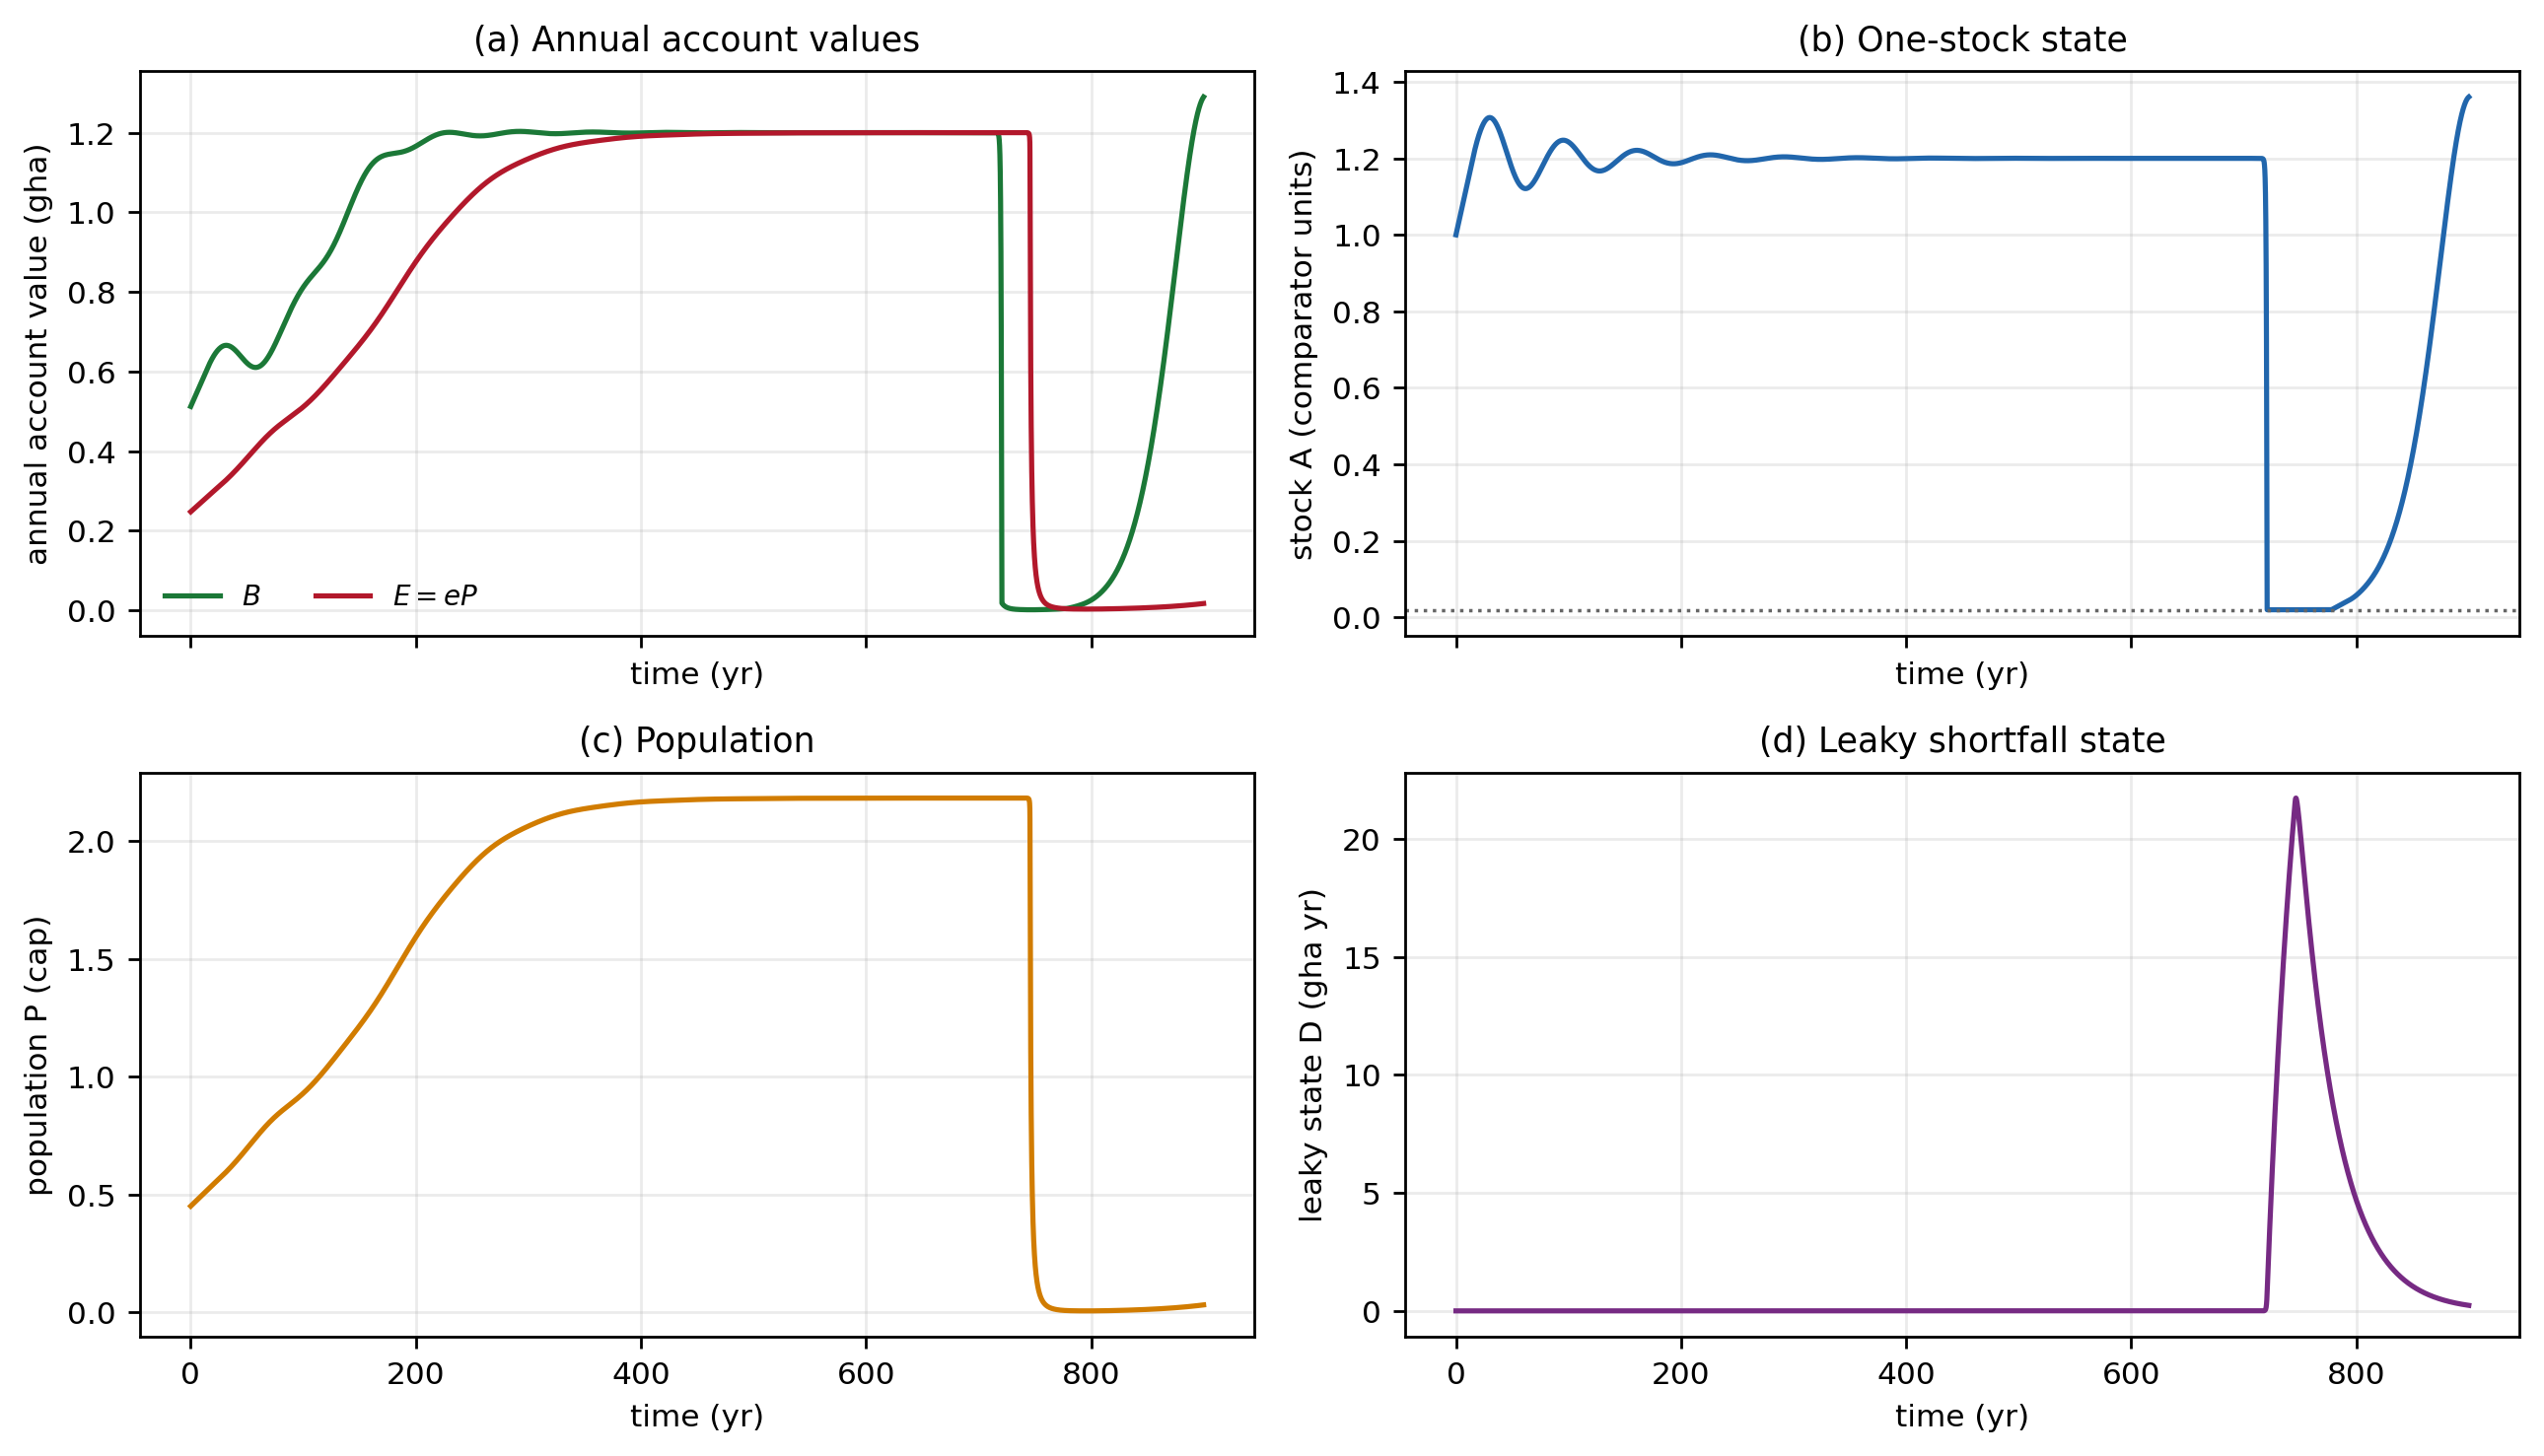
\includegraphics[width=0.96\textwidth]{si_onestock_full_trajectory}
\caption{Full delayed one-stock comparator with a logistic technology increment. Parameters are $A_0=1.0$ stock unit, $P_0=0.45$\,cap, $b_0=0.5$, $b_G=0.6$, $\rho=0.08$\,yr$^{-1}$, $A_{\max}=1.2$ stock units, $e=0.55$\,gha\,cap$^{-1}$, $r=0.02$\,yr$^{-1}$, $\eta=0.03$\,yr$^{-1}$, $\alpha=0.2$\,gha$^{-1}$\,yr$^{-1}$, $\tau_g=15$\,yr, $\tau_p=25$\,yr, $A_{\mathrm{ext}}=0.02$ stock units, $K_{\min}=10^{-4}$\,cap, $\Delta b=0.5$\,gha per stock unit, $\kappa=0.04$\,yr$^{-1}$, and $t_w=120$\,yr; $\sigma=1$, $\omega_{Tb}=1$, and $D_0=0$. The positive-part operator is exact. $B$ and $E$ are in gha, $A$ is in comparator-specific stock units, $P$ is in cap, and $D$ is in gha\,yr. The trajectory reaches the imposed lower bound near $721$\,yr, then recovers as modeled demand falls; the bound is not absorbing. This is a conditional model illustration, not an observation or a two-land result.}
\label{fig:si_onestock_full}
\end{figure}

\begin{figure}[htbp]
\centering
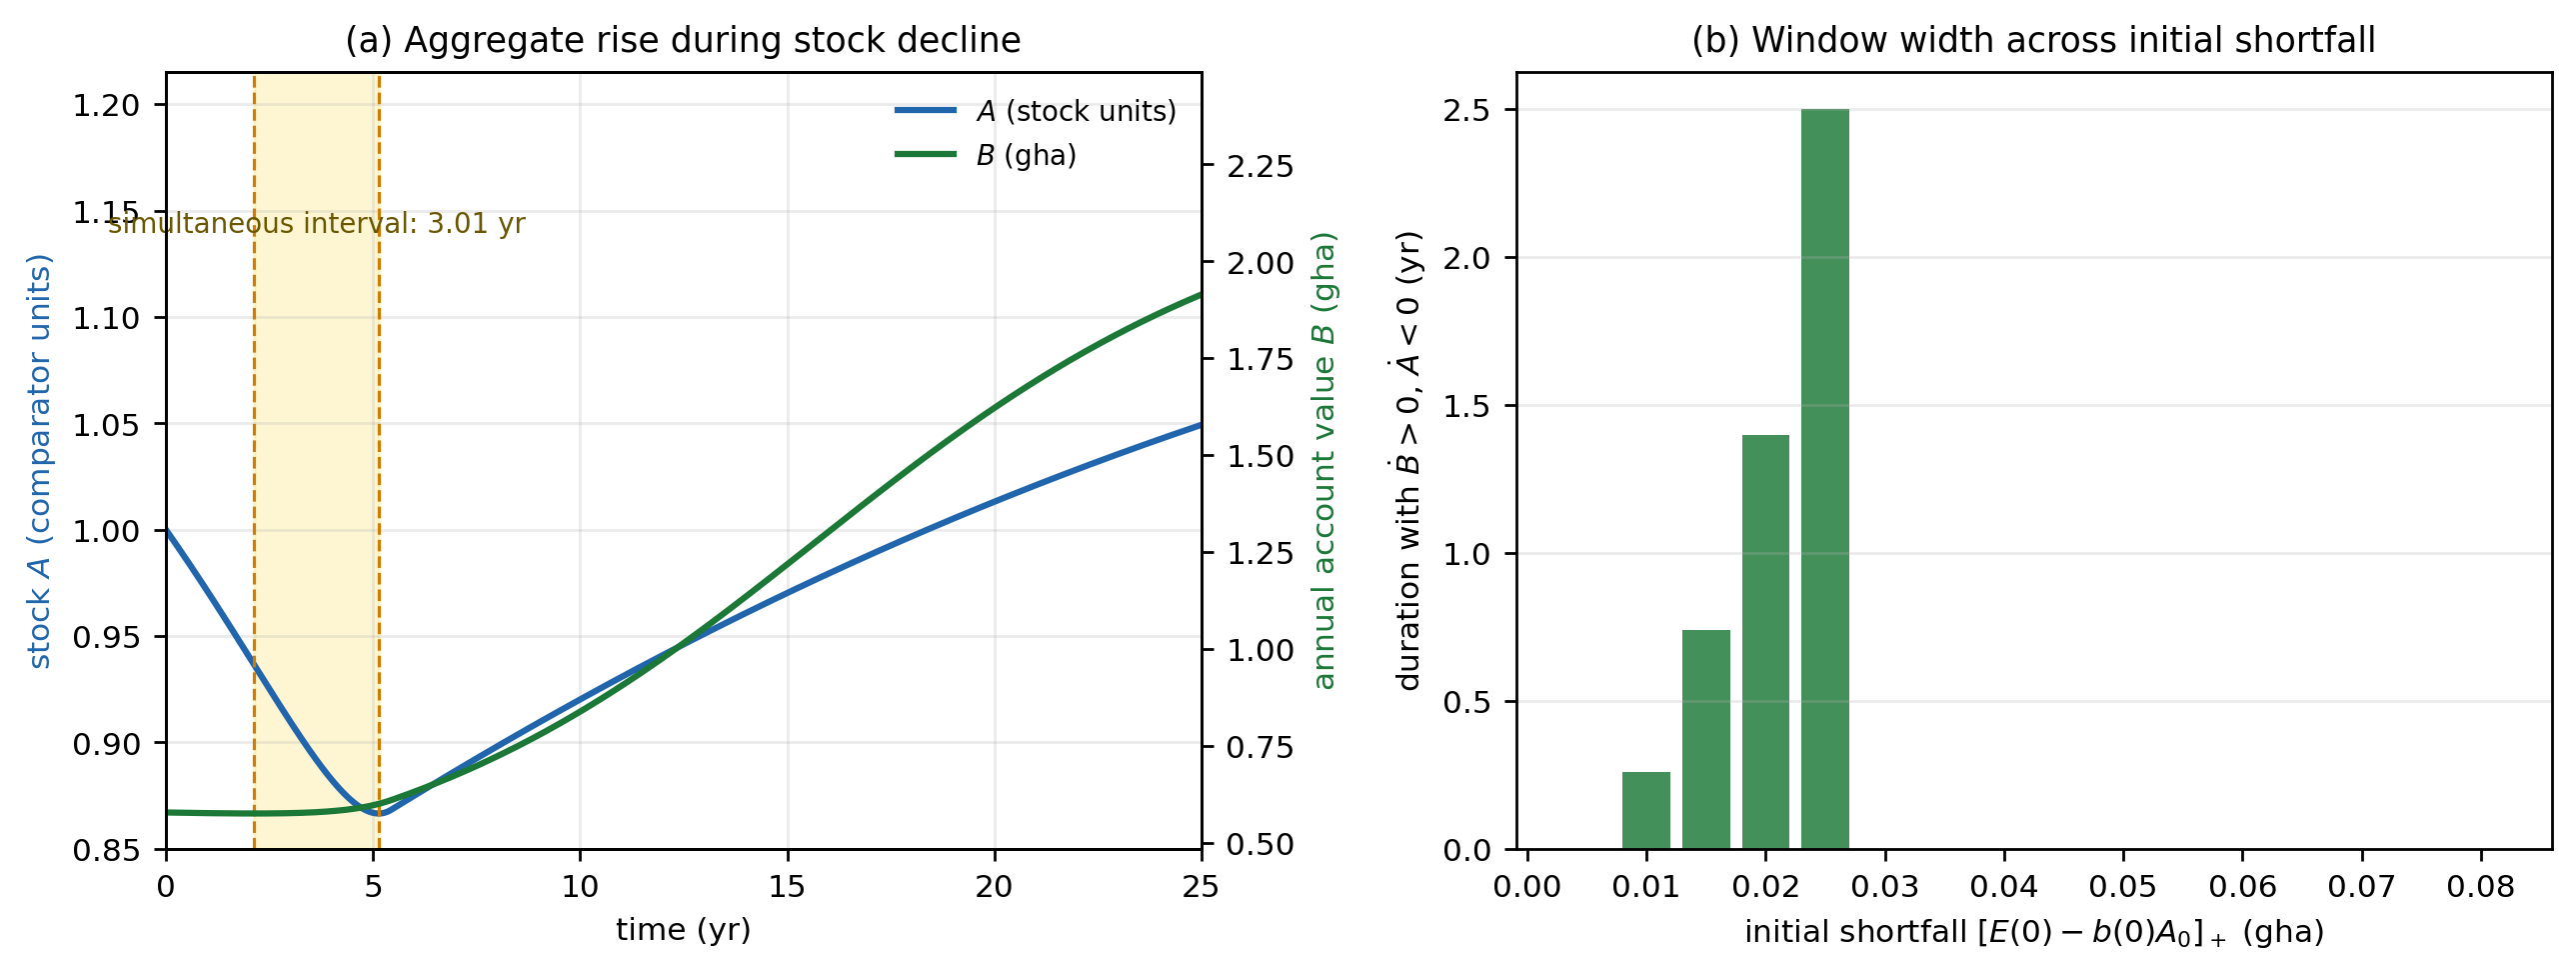
\includegraphics[width=0.96\textwidth]{si_onestock_mask_window}
\caption{One-stock masking example with fixed demand and no delays. Parameters are $A_0=1.0$ stock unit, $E=0.60$\,gha, $b_0=0.5$, $b_G=0.8$, $\rho=0.05$\,yr$^{-1}$, $A_{\max}=1.2$ stock units, $\eta=0.05$\,yr$^{-1}$, $\alpha=0.03$\,gha$^{-1}$\,yr$^{-1}$, $\Delta b=1.5$\,gha per stock unit, $\kappa=0.2$\,yr$^{-1}$, and $t_w=15$\,yr; $\sigma=1$, $\omega_{Tb}=1$, and $D_0=0$. With the exact positive-part operator, the interval with $\dot B>0$ and $\dot A<0$ lasts about $3.0$\,yr. Over that interval, $A$ falls from about $0.937$ to $0.867$ stock units while $B$ rises from about $0.575$ to $0.600$\,gha. Panel (b) shows the interval width across initial shortfalls $[E(0)-b(0)A_0]_+$ for this parameterization. These are conditional comparator outputs.}
\label{fig:si_onestock_mask}
\end{figure}

\begin{figure}[htbp]
\centering
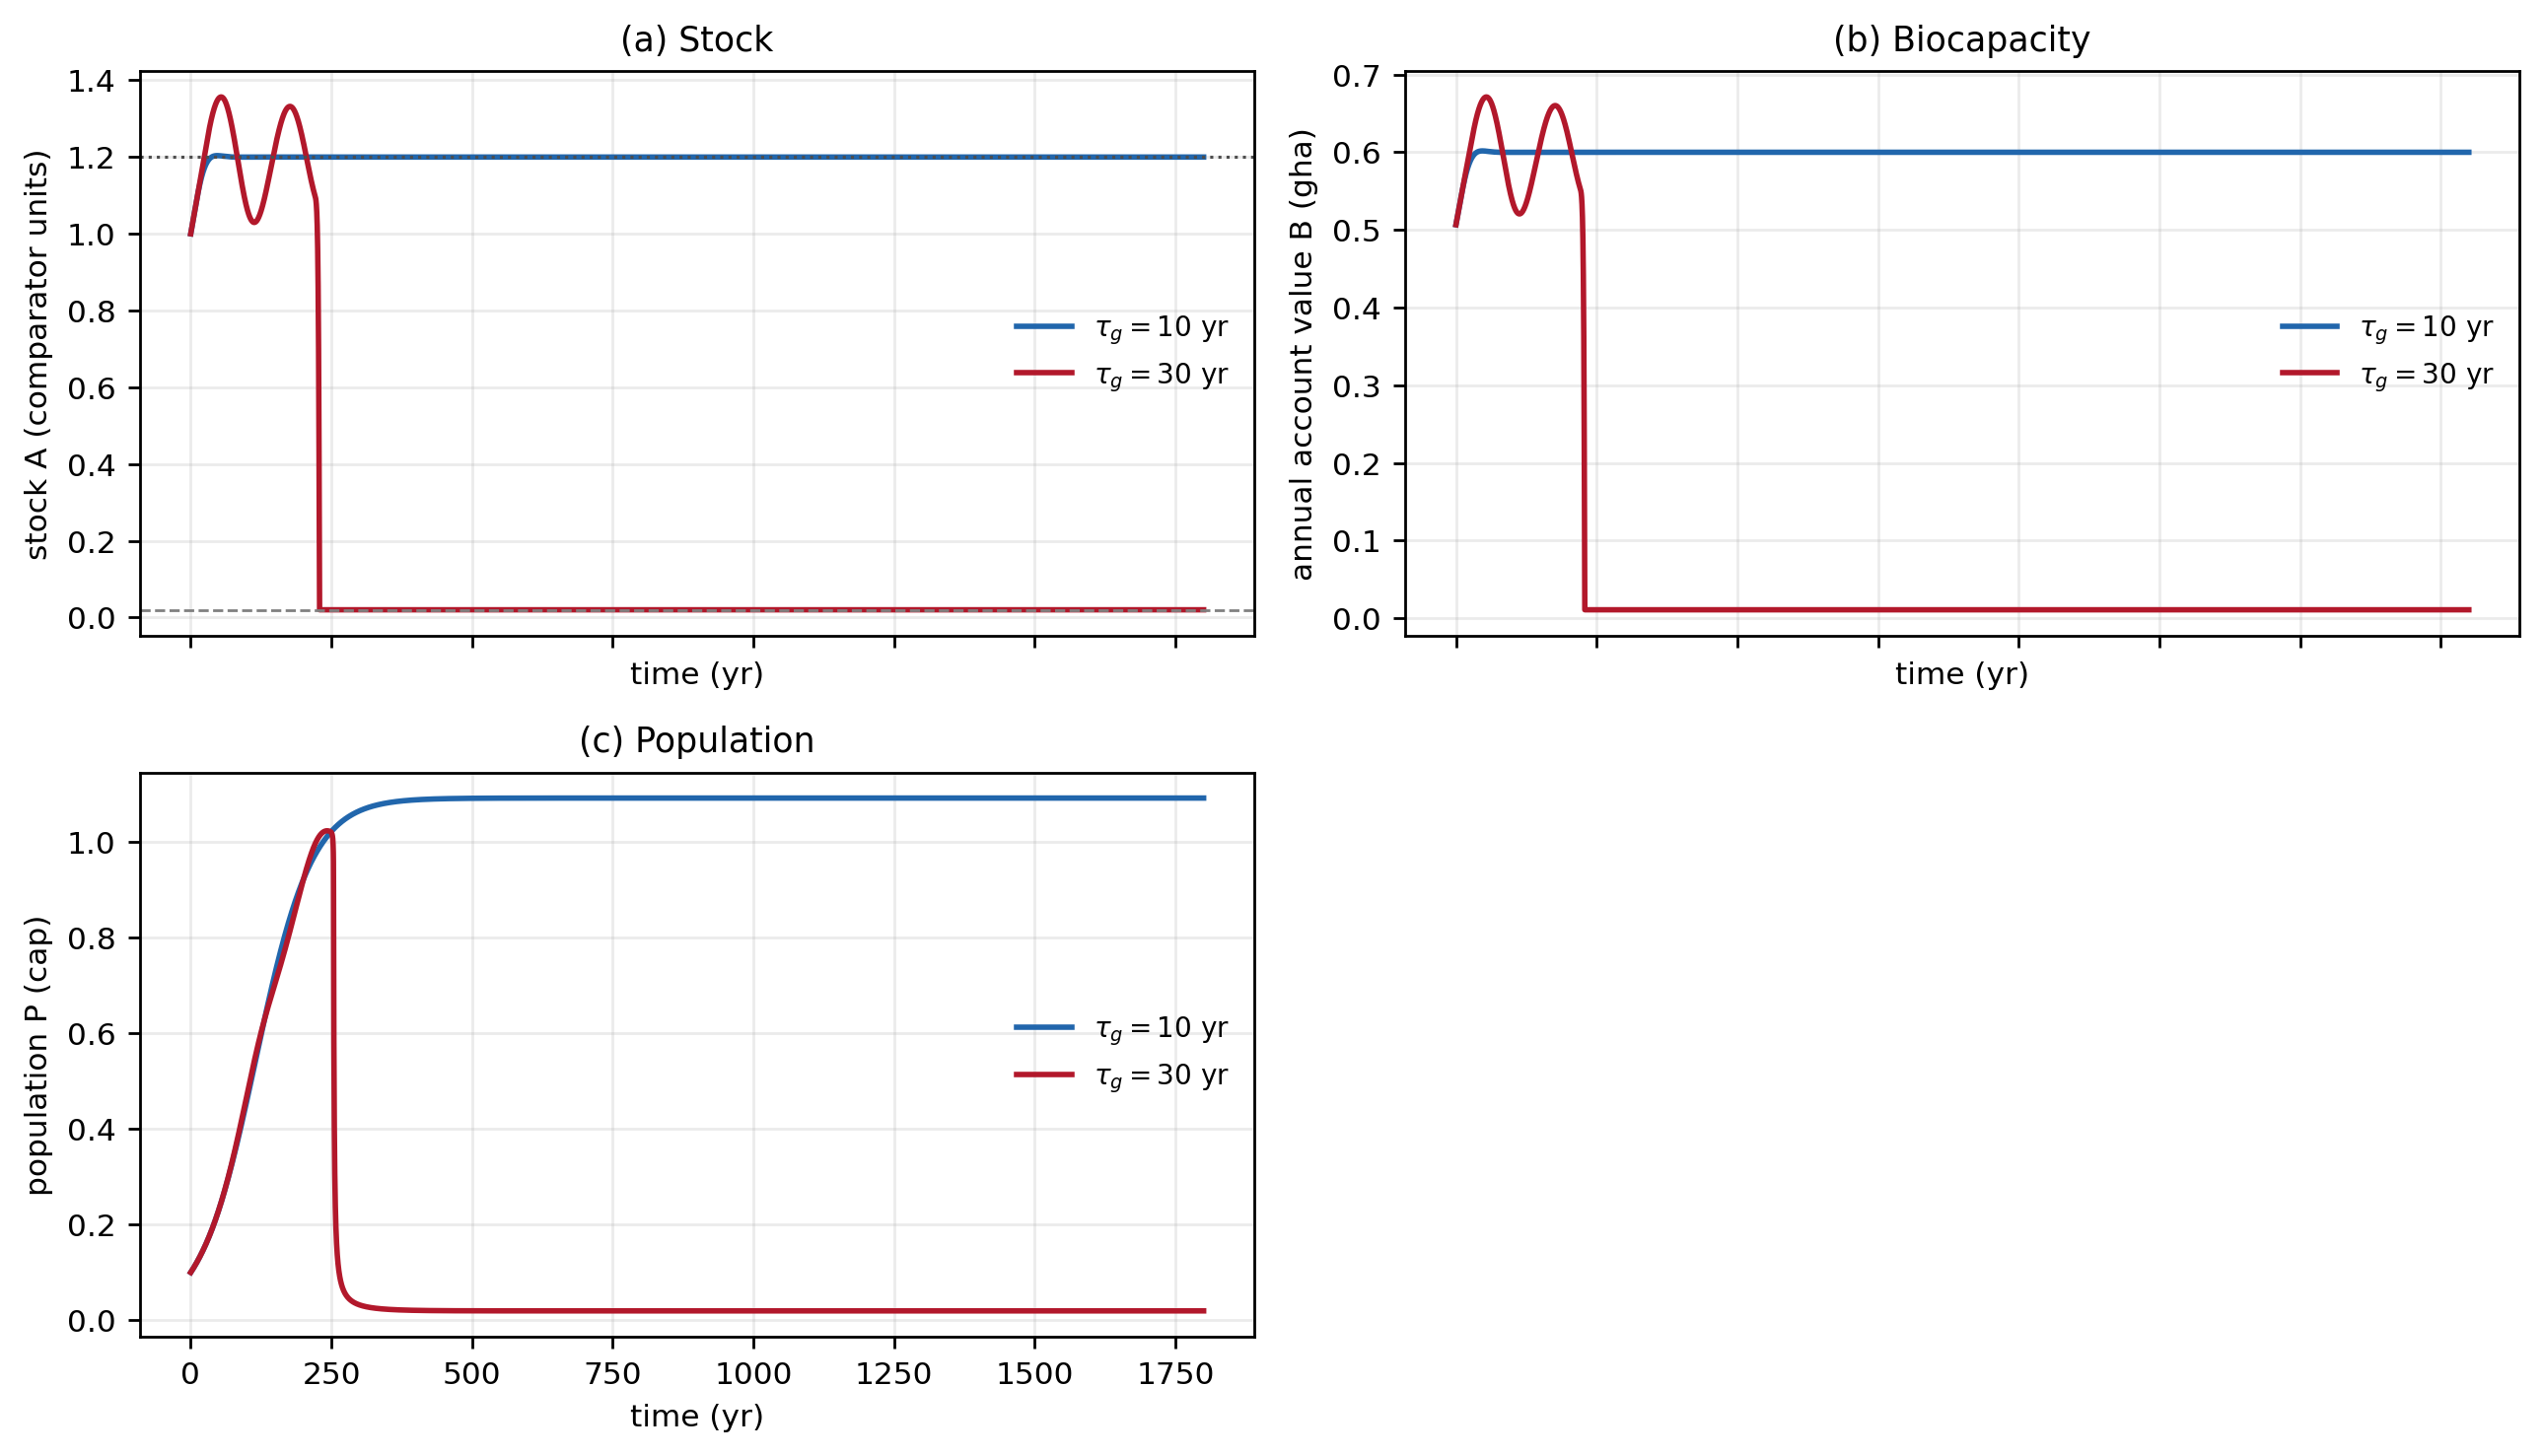
\includegraphics[width=0.96\textwidth]{si_onestock_delay_examples}
\caption{Controlled regeneration-delay examples in the debt-free one-stock subsystem. Both runs use $A_0=1.0$ stock unit, $P_0=0.1$\,cap, $b=0.5$, $b_G=0.8$, $\rho=0.05$\,yr$^{-1}$, $A_{\max}=1.2$ stock units, $e=0.55$\,gha\,cap$^{-1}$, $r=0.02$\,yr$^{-1}$, $\tau_p=25$\,yr, $A_{\mathrm{ext}}=0.02$ stock units, $K_{\min}=10^{-6}$\,cap, and $\sigma=1$; only $\tau_g$ differs ($10$ versus $30$\,yr). $B$ is in gha, $P$ in cap, and $A$ in comparator-specific stock units. These selected trajectories do not establish a general critical delay.}
\label{fig:si_onestock_delay}
\end{figure}

\begin{figure}[htbp]
\centering
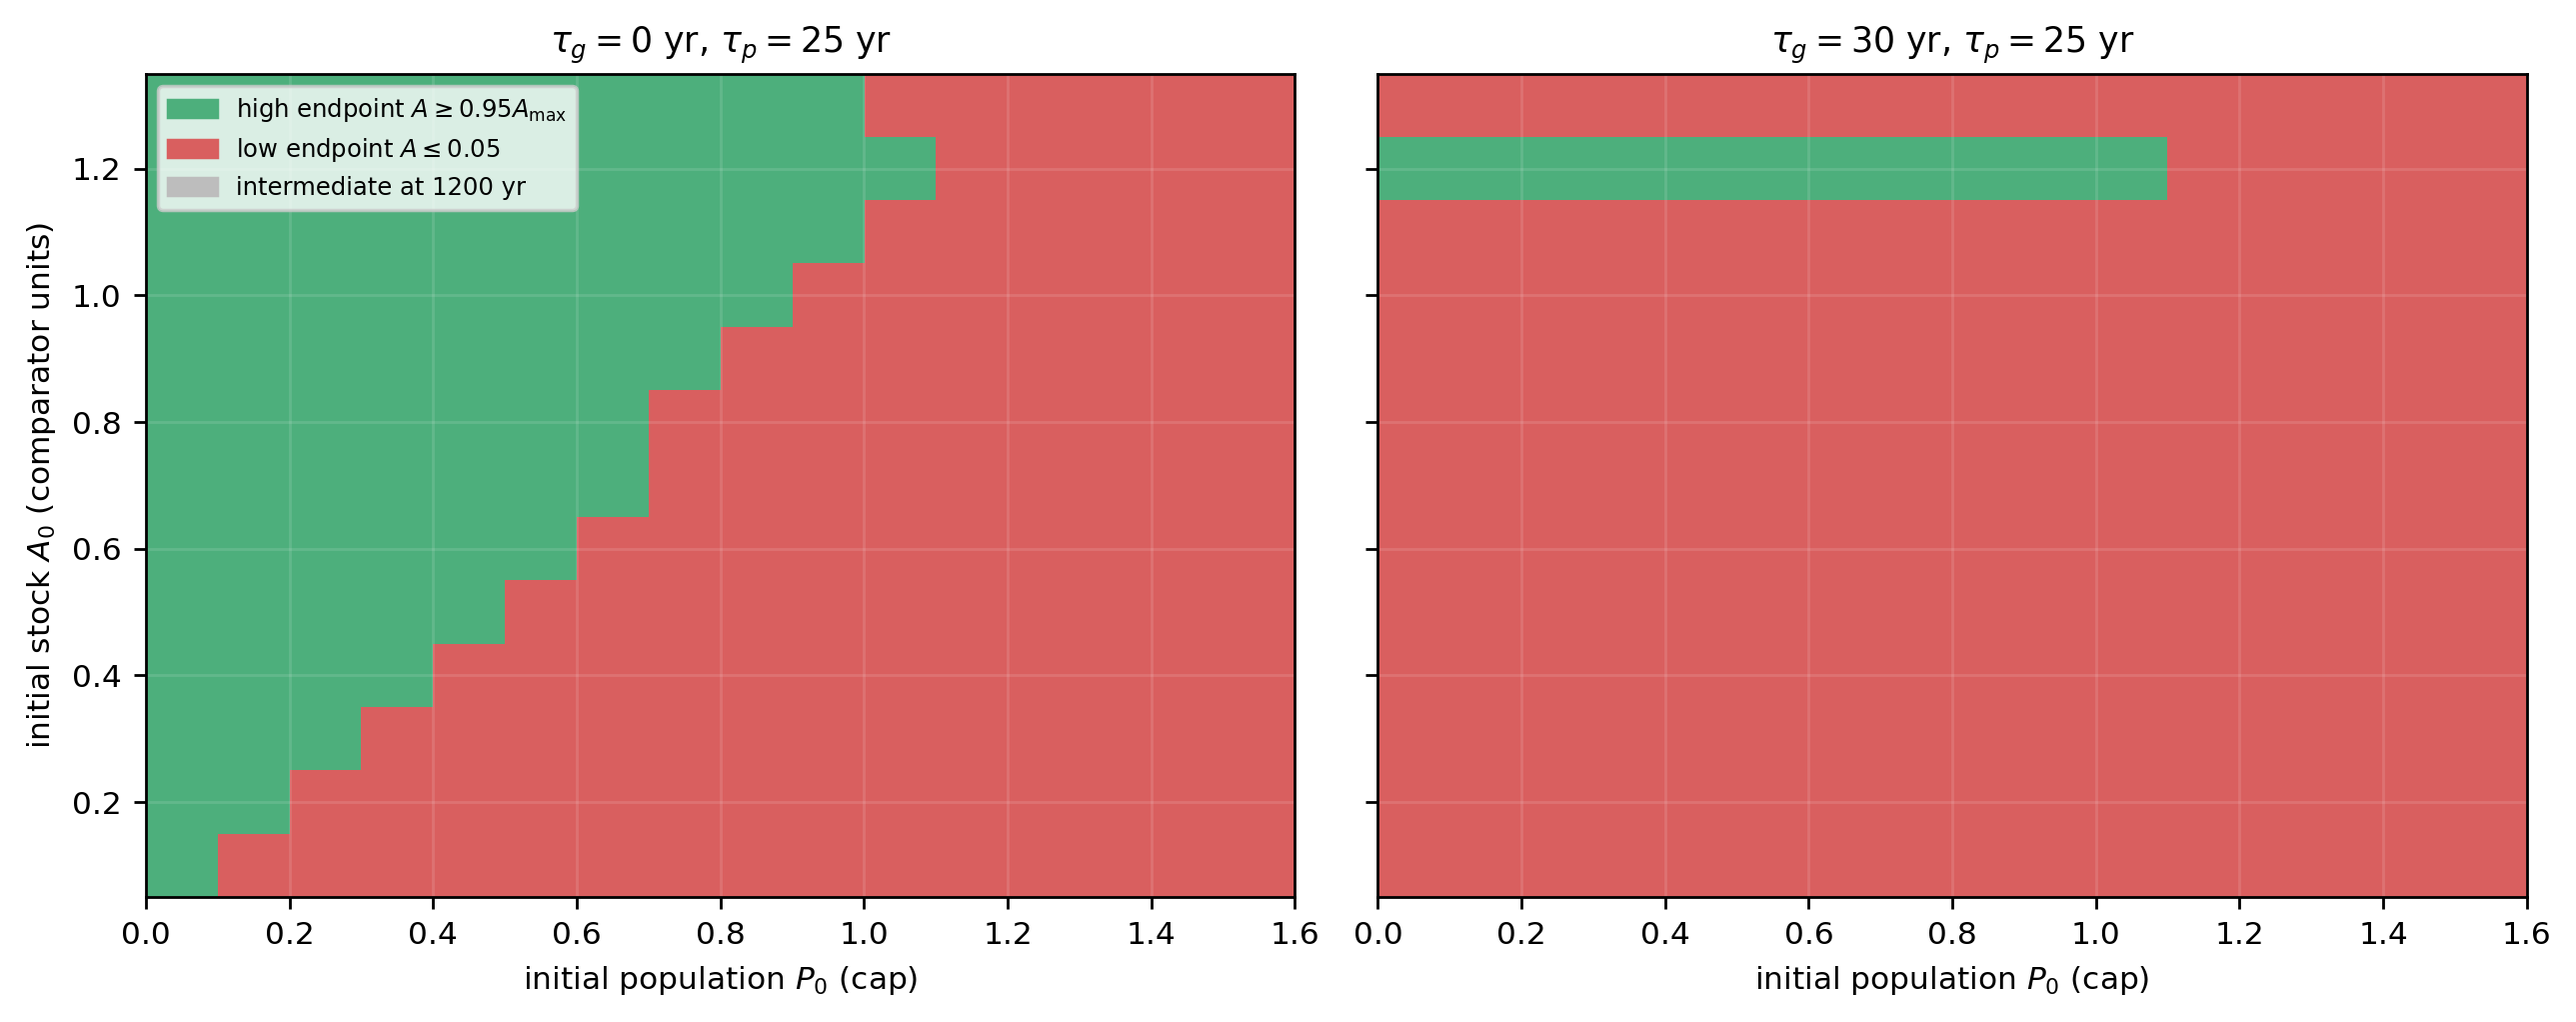
\includegraphics[width=0.96\textwidth]{si_onestock_basin}
\caption{Finite-grid initial-condition classification in the debt-free one-stock subsystem. The runs use the parameter set in Fig.~\ref{fig:si_onestock_delay}, with $K_{\min}=10^{-6}$\,cap and $\tau_p=25$\,yr; $\tau_g=0$\,yr in the left panel and $30$\,yr in the right. The imposed lower bound is $A_{\mathrm{ext}}=0.02$ stock units. The grid uses $A_0=0.10,0.20,\ldots,1.30$ stock units and $P_0=0.05,0.15,\ldots,1.55$\,cap; trajectories run to $1200$\,yr with $\Delta t=0.5$\,yr. Green marks a high endpoint $A(1200)\ge0.95A_{\max}$, red a low endpoint $A(1200)\le0.05$ stock units, and gray an intermediate endpoint. These display-grid categories are not probabilities or continuous-basin measures.}
\label{fig:si_onestock_basin}
\end{figure}

\section{Controlled technology-wave experiment}\label{si:tbwave}

The matched experiment compares endogenous-demand runs with the technology increment $T_b$ switched on or off, at $P_0=1.0$ or $1.2$\,cap. Within each pair, the runs share $A_{tot}=2.5$\,ha, $A_{f0}=0.6$\,ha, $A_{c0}=0.9$\,ha, $q_0=0.9$, and $D_0=0.0$\,gha\,yr. Parameters and numerical methods are matched; only $\omega_{Tb}$ differs. Both runs also share constant pre-run histories at $q_0=0.9$ and the no-wave initial account value $B=0.560184$\,gha.

Shared parameter values are $b_{f0}=0.85$\,gha\,ha$^{-1}$, $b_c=0.05$\,gha\,ha$^{-1}$, $b_{G,c}=0.8$\,gha\,yr\,ha$^{-1}$, $\rho_c=0.08$\,yr$^{-1}$, $\alpha=0.03$\,gha$^{-1}$\,yr$^{-1}$, $\eta=0.05$\,yr$^{-1}$, $\eta_f=0.05$\,yr$^{-1}$, $\mu=0.06$\,yr$^{-1}$, $e=0.55$\,gha\,cap$^{-1}$, $r=0.02$\,yr$^{-1}$, $\tau_g=20$\,yr, $\tau_p=25$\,yr, $\tau_{conv}=1$\,yr, and $\chi_r=0.10$\,gha$^{-1}$\,yr$^{-1}$. The active wave uses $\Delta b=1.0$\,gha\,ha$^{-1}$, $\kappa_w=0.1$\,yr$^{-1}$, and $t_{wave}=40$\,yr; runs last $250$\,yr. The logistic increment is already nonzero at $t=0$ ($T_b(0)=0.017986$\,gha\,ha$^{-1}$), so initial $B$ is $0.560184$\,gha without the wave and $0.570976$\,gha with it. This small difference comes from the logistic tail. Land, quality, population, and debt states otherwise match, and the pre-run $B$ history remains common. The wave reaches half its increment at $t_{wave}=40$\,yr.

Figure~\ref{fig:si_wave_debt} shows the $P_0=1.0$ pair. In both runs, peak debt occurs after the wave midpoint: $D_{max}=0.008126$\,gha\,yr at $86.15$\,yr without the wave and $0.020205$\,gha\,yr at $115.60$\,yr with it. At $P_0=1.2$, the all-time maximum occurs early and is lower with the wave, but the maximum for $t\ge t_{wave}$ is higher. Table~\ref{tab:si_wave_debt} reports both windows. Because $t_{wave}$ marks the logistic midpoint, the post-midpoint window includes the wave's continued rise.

\begin{table}[htbp]
\centering\small
\caption{Matched technology-wave/no-wave debt maxima. Entries are $D_{max}$ in gha\,yr, with the time of the maximum in years in parentheses; the ratio is wave/no-wave. ``All'' is the maximum over $0\le t\le250$\,yr; $t\ge40$ is the post-midpoint maximum. The $P_0=1.0$ all-time peaks both occur after the midpoint.}
\label{tab:si_wave_debt}
\begin{tabularx}{\textwidth}{r l r l >{\centering\arraybackslash}X >{\centering\arraybackslash}X r}
\toprule
$P_0$ (cap) & quality update & $\Delta t$ (yr) & window & no wave $D_{max}$ (time) & wave $D_{max}$ (time) & ratio \\
\midrule
$1.0$ & delayed & $0.050$ & all & $0.008126\ (86.15)$ & $0.020205\ (115.60)$ & $2.487$ \\
$1.0$ & delayed & $0.025$ & all & $0.008105\ (86.20)$ & $0.020195\ (115.65)$ & $2.492$ \\
$1.0$ & current & $0.050$ & all & $0.008326\ (85.70)$ & $0.020168\ (115.60)$ & $2.422$ \\
$1.2$ & delayed & $0.050$ & all & $0.061218\ (1.65)$ & $0.051037\ (1.45)$ & $0.834$ \\
$1.2$ & delayed & $0.050$ & $t\ge40$ & $0.010854\ (81.70)$ & $0.025184\ (112.55)$ & $2.320$ \\
$1.2$ & delayed & $0.025$ & all & $0.060732\ (1.625)$ & $0.050582\ (1.475)$ & $0.833$ \\
$1.2$ & delayed & $0.025$ & $t\ge40$ & $0.010808\ (81.775)$ & $0.025165\ (112.625)$ & $2.328$ \\
\bottomrule
\end{tabularx}
\end{table}

For $P_0=1.0$, the all-time wave/no-wave peak-debt ratio is $2.487$ at $\Delta t=0.05$\,yr and $2.492$ at $0.025$\,yr; under current-quality regeneration it is $2.422$ at $0.05$\,yr. For $P_0=1.2$, all-time ratios are $0.834$ and $0.833$, while post-midpoint ratios are $2.320$ and $2.328$. Halving the step changes debt maxima by less than $0.9\%$. In the $P_0=1.0$ pair, $A_c$ stays at or above its initial $0.9$\,ha, so this experiment illustrates a conditional delayed debt rebound, not the fixed-demand capital-land drawdown. At $P_0=1.2$, the all-time and post-midpoint maxima tell different stories. The debt variable $D$ is a leaky state driven by aggregate deficit $E-B$, not an observed NFA or physical-stock quantity.

\begin{figure}[!htbp]
\centering
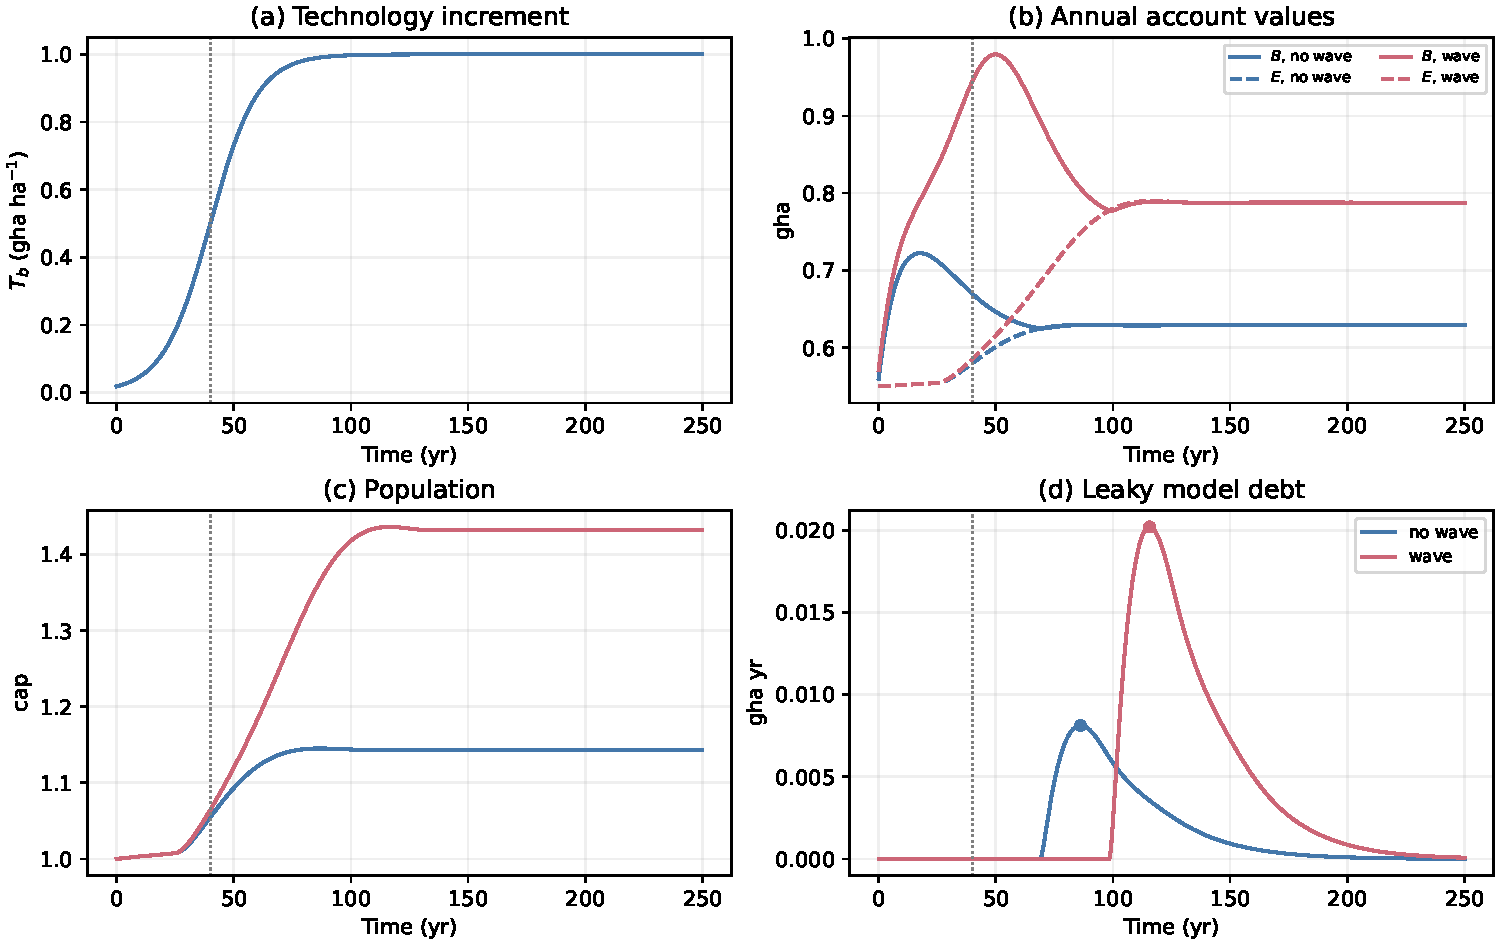
\includegraphics[width=0.92\textwidth]{fig_tb_wave_debt}
\caption{Matched endogenous-demand technology-wave/no-wave simulation at $P_0=1.0$\,cap. Parameters and initial conditions are in SI~\S S8; only $T_b$ is switched on or off. (a) The active logistic increment $T_b(t)$, with the dotted line at its midpoint $t_{wave}=40$\,yr; (b) annual account values $B$ and $E$ (gha); (c) population $P$ (cap); and (d) leaky model debt $D$ (gha\,yr). Markers denote all-time maxima: $86.15$\,yr without the wave and $115.60$\,yr with it; peak debt is $0.008126$ versus $0.020205$\,gha\,yr. The wave begins with its small logistic tail at $t=0$ and approaches $\Delta b=1.0$\,gha\,ha$^{-1}$. The dotted line marks the midpoint, not an end date.}
\label{fig:si_wave_debt}
\end{figure}

\section{Sharp static identification bounds and witnesses}\label{si:c13ident}

The intervals in main-text Proposition~4 follow from the static observation relation and the stated allocation restrictions. The independently known inputs are total area $L=A_{tot}$, minimum capital area $a_{\min}$, current fast-land yield $b_f$, and a continuously attainable, area-independent interval $[u_-,u_+]$ for $u=\Ups(q)$, with $0<u_-\le u_+<b_f$. All land is nonnegative and $A_c\ge a_{\min}$. Additional joint restrictions on yields and land allocations require projection of the corresponding joint feasible set.

\subsection{Proof and feasibility construction}

Fix $A_c=a\in[a_{\min},L]$. The remaining choices are $A_f\in[0,L-a]$ and $u\in[u_-,u_+]$, with $A_r=L-a-A_f$. The continuous affine map $b_fA_f+ua$ maps this connected rectangle onto the full interval
\[
[\,u_-a,\ b_f(L-a)+u_+a\,].
\]
Thus a compatible allocation exists exactly when $u_-a\le B\le b_f(L-a)+u_+a$. Since $b_f-u_+>0$, solving gives
\[
a_{\min}\le a\le\min\{L,B/u_-,(b_fL-B)/(b_f-u_+)\}.
\]
This is a set equality, not merely an outer bound. For an explicit construction, choose any $u$ in
\[
[u_-,u_+]\ \cap\ [(B-b_f(L-a))/a,\ B/a]
\]
when $a>0$, and set $A_f=(B-ua)/b_f$, $A_r=L-a-A_f$. The inequalities guarantee the intersection is nonempty. At $a=0$, feasibility instead requires $0\le B\le b_fL$, and $A_f=B/b_f$ supplies the construction.

When $A_f$ is independently observed, the residual $C=B-b_fA_f$ obeys $C=ua$. For $C\ge0$, intersecting $C/u_+\le a\le C/u_-$ with $[a_{\min},L-A_f]$ gives the second interval. Choosing $u=C/a$ constructs every feasible positive $a$; when $a=C=0$, any permitted $u$ works. If $C<0$, the residual is inconsistent with nonnegative capital area and positive yield. If $q$ is also independently observed, its known $\Ups(q)>0$ gives the unique feasible candidate $a=C/\Ups(q)$.

Attainment of each $u$ by an admissible quality value is essential to calling these intervals sharp. Under the baseline law $\Ups(q)=0.05+0.064q(1-q)$ on $[0,1]$, the yield image is exactly $[0.05,0.066]$\,gha\,ha$^{-1}$. Its maximum occurs at $q=0.5$; its minimum at $q=0$ or $1$. This is a readout property, not a monotonic ordering of ecological condition. In particular, $q=0.1$ and $0.9$ give the same $\Ups$, so known $\Ups$ alone does not uniquely identify $q$.

\subsection{Numerical illustration and interpretation}

For $B=0.825$\,gha, $b_f=0.85$\,gha\,ha$^{-1}$, $L=2.5$\,ha, $a_{\min}=0.05$\,ha, and the above yield interval, the $B$-only interval is $[0.05,1.6581632653\ldots]$\,ha. Independently fixing $A_f=0.785/0.85$\,ha gives $C=0.04$\,gha and $A_c\in[0.6060606061\ldots,0.8]$\,ha. Table~\ref{tab:si_c13witness} supplies endpoint witnesses. They satisfy the identical $B$ and $A_f$ constraints and respect total area; neither is asserted to be reachable from the baseline history. The lower endpoint of the wider $B$-only interval is feasible, for example, with $a=0.05$, $u=0.05$, and $A_f=(0.825-0.0025)/0.85$\,ha. Its upper endpoint is feasible at $u=0.066$, $A_r=0$.

\begin{table}[htbp]
\centering\small
\caption{Endpoint witnesses for the $B,A_f$ interval. Areas are in ha, $u$ in gha\,ha$^{-1}$, $B$ in gha, and $q$ is dimensionless. Values shown are rounded; the calculations use unrounded $A_f$.}
\label{tab:si_c13witness}
\begin{tabular}{lrrrrrr}
\toprule
Endpoint & $A_f$ & $A_c$ & $A_r$ & $q$ & $u$ & Calculated $B$ \\
\midrule
lower & 0.923529 & 0.606061 & 0.970410 & 0.5 & 0.066 & 0.825 \\
upper & 0.923529 & 0.800000 & 0.776471 & 1.0 & 0.050 & 0.825 \\
\bottomrule

\end{tabular}
\end{table}

At known $q=0.9$, $A_c=0.04/0.05576=0.7173601148\ldots$\,ha. These deterministic bounds assume exact inputs and a valid observation operator. With uncertain $B,b_f,A_f$ or yield restrictions, define a coherent joint feasible uncertainty set and project it onto $A_c$; independent endpoint combinations can otherwise be inconsistent. No empirical mapping from NFA land accounts to these physical model areas is established here. The construction narrows an identified set; it does not establish dynamic observability or make unobserved quality measurable.

\section{Integrated contribution budgets and numerical refinement}\label{si:c13budget}

\subsection{Continuous-time identity and quadrature}

Let $u=\Ups(q)$ and $M=\mu A_r-\eta_fA_f$. Differentiating the observation relation and substituting the land equations gives, almost everywhere along the absolutely continuous projected trajectory,
\[
\dot B=(b_f-u)u_c+b_fM+uR_{rc}+b_{G,c}G_c'(q)A_c\dot q+A_f\dot b_f,
\qquad
\dot b_f=e^{-\alpha D}\dot T_b-\alpha b_f\dot D.
\]
The projected quality velocity is used in this identity. Each integrand has units gha\,yr$^{-1}$ and each time integral has units gha. The fast-yield contribution comprises $A_fe^{-\alpha D}\dot T_b$ from technology and $-\alpha A_fb_f\dot D$ from debt. Debt accumulation reduces fast-land yield, whereas debt decay increases it. Their integrated contributions summarize the signed effect over the observation interval; peak debt is a separate statistic.

All five continuous-time integrands are evaluated at the numerical state nodes and integrated using the trapezoidal rule. The endpoint difference is evaluated separately from the observation relation. The signed closure residual is
\[
\varepsilon_T=B(T)-B(0)-\sum_j I_j,
\]
where $I_j$ denotes an integrated contribution. Finite-step discrepancies reflect the Euler trajectory approximation, quadrature error and the non-smooth quality constraint. Timestep refinement assesses the resulting closure error; it does not provide a uniform trajectory-error bound.

\subsection{Simulation conditions}

Four conditions are considered. The fixed-demand condition uses $A_{c0}=1.5$\,ha, $P_0=1.5$\,cap, $E=0.825$\,gha, $\chi_r=0$ and $T=100$\,yr. The restoration condition uses $A_{c0}=1.0$\,ha, $P_0=2.0$\,cap, $E=eP$, $\chi_r=0.1$\,gha$^{-1}$\,yr$^{-1}$ and $T=400$\,yr. The control and technology conditions use $A_{c0}=0.9$\,ha, $P_0=1.0$\,cap, endogenous demand, $\chi_r=0.1$\,gha$^{-1}$\,yr$^{-1}$ and $T=250$\,yr; only the technology condition includes the logistic yield increment specified in S8. All conditions share $A_{f0}=0.6$\,ha, $q_0=0.9$, $D_0=0$, $A_{tot}=2.5$\,ha and the baseline coefficients and delays. Population evolves in the fixed-demand condition, but demand remains exogenous.

At each Euler step, the current state is evaluated at the preceding node, while the technology input and delayed observations are evaluated at the right endpoint. Current supply is calculated on the preceding state using that technology input; post-update supply is stored for subsequent delayed interpolation. The pre-run quality history is constant at $0.9$. Pre-run supply is the no-technology initial value, including in the matched technology comparison. The quality velocity is projected before updating, followed by clipping to the admissible interval. Nonnegative bounds are imposed on $A_f,P,D$, and $A_c\ge0.05$\,ha. Reserve area is calculated from total-area conservation and monitored. The optional fast-land ceiling is inactive.

At $\Delta t=0.05$\,yr, peak debt is $0.0081259288$\,gha\,yr at $86.15$\,yr in the control condition and $0.0202046739$\,gha\,yr at $115.60$\,yr in the technology condition (Figure~\ref{fig:si_wave_debt}). The contribution integrals use the same mathematical model and history specifications as these simulations.

\subsection{Contribution integrals and closure}

Table~\ref{tab:si_c13budget} reports integrated contributions at the smallest timestep. Table~\ref{tab:si_c13split} separates technology and debt within the fast-yield contribution. The positive technology contribution is substantially offset by the negative maintenance--retirement contribution along the technology trajectory. These are decompositions of coupled model trajectories, not estimates of empirical causal effects. The direct restoration contribution to $B$ is distinct from restoration's total effect on the evolving state.

\begin{table}[htbp]
\centering\small
\setlength{\tabcolsep}{4pt}
\caption{Integrated contributions to model biocapacity in gha at $\Delta t=0.00078125$\,yr. Horizons are 100 yr for fixed demand, 400 yr for restoration, and 250 yr for the control and technology conditions. Residuals are the endpoint change minus the sum of integrated contributions.}
\label{tab:si_c13budget}
\begin{tabular}{lrrrr}
\toprule
Contribution or statistic & Fixed demand & Restoration & Control & Technology \\
\midrule
Conversion & +0.547925 & +0.513933 & +0.016593 & +0.042011 \\
Maintenance/retirement & -0.311098 & -0.218037 & +0.037254 & -0.487030 \\
Restoration & +0.000000 & +0.016561 & +0.020431 & +0.046986 \\
Quality readout & -0.006470 & -0.002577 & -0.005498 & -0.005567 \\
Fast-yield change & +0.000873 & +0.002687 & +0.000001 & +0.620615 \\
Sum of integrals & +0.231230 & +0.312567 & +0.068781 & +0.217016 \\
$B(T)-B(0)$ & +0.231310 & +0.312764 & +0.068791 & +0.217025 \\
Closure residual & +0.000080 & +0.000197 & +0.000010 & +0.000008 \\
\bottomrule

\end{tabular}
\end{table}

\begin{table}[htbp]
\centering\small
\caption{Technology and debt components of the fast-yield integral, in gha, at the smallest timestep. A small signed debt integral is compatible with nonzero debt at intermediate times.}
\label{tab:si_c13split}
\begin{tabular}{lrrr}
\toprule
Condition & Technology & Debt & Fast-yield total \\
\midrule
Fixed demand & +0.00000000 & +0.00087257 & +0.00087257 \\
Restoration & +0.00000000 & +0.00268738 & +0.00268738 \\
Control & +0.00000000 & +0.00000057 & +0.00000057 \\
Technology & +0.62061305 & +0.00000241 & +0.62061546 \\
\bottomrule

\end{tabular}
\end{table}

Seven nested timesteps are used: $0.05$, $0.025$, $0.0125$, $0.00625$, $0.003125$, $0.0015625$ and $0.00078125$\,yr. At the smallest timestep, absolute closure residuals relative to the endpoint changes are $0.0348\%$, $0.0628\%$, $0.0143\%$ and $0.00380\%$ for fixed demand, restoration, control and technology, respectively. These satisfy the closure tolerance $|\varepsilon_T|/|\Delta B|<0.001$. Absolute residuals decrease at every tested timestep halving in all four conditions (Table~\ref{tab:si_c13refine}). Maximum differences between nested-grid solutions for $A_c,B,D$ are provided with the computational data.

\clearpage
{\small
\begin{longtable}{lrrrr}
\caption{Timestep refinement of the integrated contribution budget. $\Delta B$, $\sum I_j$ and $\varepsilon_T=\Delta B-\sum I_j$ are in gha; timestep is in yr.}\label{tab:si_c13refine}\\
\toprule
Condition & $\Delta t$ & $\Delta B$ & $\sum I_j$ & $\varepsilon_T$ \\
\midrule
\endfirsthead
\toprule
Condition & $\Delta t$ & $\Delta B$ & $\sum I_j$ & $\varepsilon_T$ \\
\midrule
\endhead
Fixed demand & 0.05000000 & +0.23131065 & +0.22616616 & +5.144e-03 \\
Fixed demand & 0.02500000 & +0.23131037 & +0.22873531 & +2.575e-03 \\
Fixed demand & 0.01250000 & +0.23131023 & +0.23002006 & +1.290e-03 \\
Fixed demand & 0.00625000 & +0.23131016 & +0.23066538 & +6.448e-04 \\
Fixed demand & 0.00312500 & +0.23131012 & +0.23098805 & +3.221e-04 \\
Fixed demand & 0.00156250 & +0.23131010 & +0.23114939 & +1.607e-04 \\
Fixed demand & 0.00078125 & +0.23131009 & +0.23122970 & +8.040e-05 \\
Restoration & 0.05000000 & +0.31300381 & +0.30043090 & +1.257e-02 \\
Restoration & 0.02500000 & +0.31288178 & +0.30659261 & +6.289e-03 \\
Restoration & 0.01250000 & +0.31282082 & +0.30967470 & +3.146e-03 \\
Restoration & 0.00625000 & +0.31279032 & +0.31121731 & +1.573e-03 \\
Restoration & 0.00312500 & +0.31277507 & +0.31198869 & +7.864e-04 \\
Restoration & 0.00156250 & +0.31276745 & +0.31237439 & +3.931e-04 \\
Restoration & 0.00078125 & +0.31276363 & +0.31256709 & +1.965e-04 \\
Control & 0.05000000 & +0.06881854 & +0.06818752 & +6.310e-04 \\
Control & 0.02500000 & +0.06880431 & +0.06848617 & +3.181e-04 \\
Control & 0.01250000 & +0.06879720 & +0.06863550 & +1.617e-04 \\
Control & 0.00625000 & +0.06879364 & +0.06871312 & +8.052e-05 \\
Control & 0.00312500 & +0.06879187 & +0.06875193 & +3.993e-05 \\
Control & 0.00156250 & +0.06879098 & +0.06877134 & +1.964e-05 \\
Control & 0.00078125 & +0.06879053 & +0.06878067 & +9.860e-06 \\
Technology & 0.05000000 & +0.21685345 & +0.21632588 & +5.276e-04 \\
Technology & 0.02500000 & +0.21694039 & +0.21667384 & +2.666e-04 \\
Technology & 0.01250000 & +0.21698384 & +0.21684782 & +1.360e-04 \\
Technology & 0.00625000 & +0.21700556 & +0.21693788 & +6.768e-05 \\
Technology & 0.00312500 & +0.21701642 & +0.21698291 & +3.351e-05 \\
Technology & 0.00156250 & +0.21702185 & +0.21700543 & +1.642e-05 \\
Technology & 0.00078125 & +0.21702456 & +0.21701631 & +8.251e-06 \\
\bottomrule

\end{longtable}
}

The numerical bounds on $A_f,A_c,P,D$ require no clipping in these 28 simulations, and the conversion-availability constraint is inactive. Each simulation contains one finite-step overshoot of the quality ceiling followed by clipping. At the smallest timestep, the maximum pre-clipping overshoot is $1.25\times10^{-6}$, and the first constrained node occurs at $13.8890625$\,yr. Minimum reserve areas are $0.400000$, $0.775769$, $0.531279$ and $0.286300$\,ha for fixed demand, restoration, control and technology, respectively; all exceed the monitored $0.1$\,ha threshold. Total area is conserved to floating-point precision.

For the restoration condition at $\Delta t=0.00078125$\,yr, $\min A_c=0.401217$\,ha and $A_c(400)=0.678295$\,ha, indicating partial recovery. The $\Delta t=0.1$\,yr estimates are given in Table~\ref{tab:si_recovery}. Quality trajectories for the specified $20$ and $40$\,yr delays coincide because the quality constraint is reached before either delay elapses (S2.3 and S3). The budget calculations therefore provide no additional inference about sensitivity to alternative quality histories.

The computational data contain full-precision contribution integrals, signed closure residuals, state-constraint statistics and nested-grid comparisons. Trajectories and cumulative integrals are reported at $0.05$\,yr intervals; integration uses every simulation node.

\section*{Supplementary references}
\begin{thebibliography}{99}
\small
\bibitem[{Abaee(2026a)}]{Abaee2026a} Abaee, A. (2026a). \emph{Governance delay and the stability of harvested stocks: mobilising and protective feedback rules, and the review interval as a design parameter}. Working paper. \href{https://github.com/MIKEAA2020/general-sustainability/blob/2efaa62083f2007dec3446c15c475af88f0925f3/arena%20agent%201/paper%20rewrites/latex/paper4_delay_dynamics_v41.pdf}{Manuscript}.
\bibitem[{Abaee(2026b)}]{Abaee2026b} Abaee, A. (2026b). \emph{Aggregation is a claim, not a presentation: the geometry of the acceptance gap between compensatory and noncompensatory transition assessment}. Working paper. \href{https://github.com/MIKEAA2020/general-sustainability/blob/2efaa62083f2007dec3446c15c475af88f0925f3/arena%20agent%201/paper%20rewrites/latex/paper06_assessment_separation_v71.pdf}{Manuscript}.
\bibitem[{Global Footprint Network(2009)}]{GFNStandards2009} Global Footprint Network (2009). \emph{Ecological Footprint Standards 2009}. Global Footprint Network. \url{https://www.footprintnetwork.org/content/uploads/2019/05/Ecological_Footprint_Standards_2009.pdf}.
\bibitem[{Global Footprint Network(2019)}]{GFNGuidebook2019} Global Footprint Network (2019). \emph{Working Guidebook to the National Footprint Accounts 2019}. Global Footprint Network. \url{https://www.footprintnetwork.org/content/uploads/2019/05/National_Footprint_Accounts_Guidebook_2019.pdf}.
\bibitem[{Hutchings and Reynolds(2004)}]{HutchingsReynolds2004} Hutchings, J. A. \& Reynolds, J. D. (2004). Marine fish population collapses: consequences for recovery and extinction risk. \emph{BioScience}, 54(4), 297--309.
\bibitem[{Lo et al.(2026)}]{Lo2026NFA} Lo, K., Basnet, N., Miller, E., Srikanthalingam, B., Foley, B., Van Berkum, J. L., Long, A. H., Toneva, P., Ermina, M. \& Klinkenberg, C. (2026). \emph{National Ecological Footprint and Biocapacity Accounts, Edition 2026 (1961--2025): Results and metadata, version 1.0.} Prepared for Footprint Data Foundation by researchers at York University and the University of Iceland. Workbook: \url{https://footprint.info.yorku.ca/files/2026/04/NEFBA_Data_global_national_ecological_footprint_biocapacity.xlsx}; release notes: \url{https://footprint.info.yorku.ca/files/2026/04/NEFBA_ReleaseNotes.pdf}; data page: \url{https://footprint.info.yorku.ca/data/}.
\bibitem[{Neubauer et al.(2013)}]{Neubauer2013} Neubauer, P., Jensen, O. P., Hutchings, J. A. \& Baum, J. K. (2013). Resilience and recovery of overexploited marine populations. \emph{Science}, 340(6130), 347--349.
\bibitem[{Our~World~in~Data(2026a)}]{OWIDCereal2026} Our~World~in~Data (2026a). \emph{Cereal yield.} FAOSTAT data accessed through Our World in Data; grapher page last updated 25 February 2026; accessed 24 October 2026. \url{https://ourworldindata.org/grapher/cereal-yield}.
\bibitem[{Our~World~in~Data(2026b)}]{OWIDCropland2026} Our~World~in~Data (2026b). \emph{Cropland area.} FAOSTAT data accessed through Our World in Data; grapher page last updated 25 February 2026; accessed 24 October 2026. \url{https://ourworldindata.org/grapher/cropland-area}.
\bibitem[{Poeplau et al.(2011)}]{Poeplau2011} Poeplau, C., et al. (2011). Temporal dynamics of soil organic carbon after land-use change in the temperate zone--carbon response functions as a model approach. \emph{Global Change Biology}, 17(7), 2415--2427.
\bibitem[{Poorter et al.(2016)}]{Poorter2016} Poorter, L., et al. (2016). Biomass resilience of Neotropical secondary forests. \emph{Nature}, 530(7590), 211--214.
\bibitem[{United Nations et al.(2021)}]{UN2021SEEA_EA} United Nations et al. (2021). \emph{System of Environmental-Economic Accounting---Ecosystem Accounting (SEEA EA).} White cover publication, pre-edited text subject to official editing. New York: United Nations. \url{https://seea.un.org/ecosystem-accounting}.
\end{thebibliography}

\end{document}
